

\chapter{Atari Benchmark (Experiment 2)}
\label{chap:exp2}

This chapter scales the comparison from Experiment~1 to pixel-based Atari games, narrowing the algorithm set to DQN and PPO and switching to GPU training with convolutional policies. The evaluation uses the same metrics framework from Section~\ref{sec:eval-framework}. The headline finding is that PPO solves Pong while DQN edges Breakout, but the cross-environment aggregate at $M=2$ environments is fragile and heavily dominated by whichever per-environment gap is larger. This motivates the extended study in Chapter~\ref{chap:exp3}.

The previous chapter evaluated five algorithms on three classic-control
environments using MLP policies on CPU, with bitwise-reproducible
deterministic seeding. This chapter scales the comparison to
pixel-based Atari games, narrowing the algorithm set to the two
most representative families---DQN (off-policy, value-based) and PPO
(on-policy, actor--critic)---and training with convolutional neural
networks on GPU. I wanted to test whether the DQN-vs-PPO
relationship observed in Experiment~1 holds when the observation space
shifts from low-dimensional vectors to raw pixel frames processed by
CNNs. I begin with the experimental setup and hypotheses, then present
per-environment and cross-environment results, and close with a
discussion of what matched my expectations and what surprised me.

%% ------------------------------------------------------------------
\section{Experimental Setup}
\label{sec:atari-setup}

\subsection{Hardware and Software}
\label{sec:atari-hardware}

All experiments were conducted on the same workstation used in
Experiment~1 (Table~\ref{tab:hardware}), but this time the GPU was
actively used for training. Table~\ref{tab:atari-hardware} summarises
the configuration.

\begin{table}[htbp!]
\centering
\caption{Hardware and software configuration for Experiment~2.}
\label{tab:atari-hardware}
\begin{tabular}{ll}
\toprule
\textbf{Component}   & \textbf{Specification} \\
\midrule
CPU         & AMD Ryzen 7 7800X3D (8C/16T, Zen 4, 5.05\,GHz boost) \\
GPU         & NVIDIA RTX 4090 24\,GB (\emph{used for CnnPolicy training}) \\
RAM         & 32\,GiB DDR5 \\
Storage     & WD BLACK SN850X NVMe (4\,TB + 1\,TB) \\
OS          & Arch Linux, kernel 6.18.7-zen \\
Framework   & Stable-Baselines3 v2.7.1 \citep{raffin2021sb3} \\
Backend     & PyTorch 2.10.0, Python 3.10 \\
\bottomrule
\end{tabular}
\end{table}

\subsection{Why GPU Training}
\label{sec:why-gpu}

Unlike Experiment~1, where small MLP policies made GPU offloading
counterproductive, Atari environments require convolutional forward
and backward passes on $84\times84\times4$ frame stacks. The RTX~4090
provides a massive speedup for these operations compared to CPU-only
execution.

This shift has a reproducibility trade-off. PyTorch's deterministic
mode guarantees bitwise reproducibility only on CPU; GPU kernel
scheduling introduces non-deterministic floating-point accumulation
order \citep{pytorch_reproducibility}. Both experiments use multiple
independent seeds for statistical validity, but Experiment~1
additionally achieves bitwise determinism---any researcher can re-run a
seed and obtain identical results. I compensated for the loss of bitwise
reproducibility by relying entirely on the 10-seed ensemble and its
resulting confidence intervals to establish robust conclusions.

\subsection{Algorithms, Environments, and Protocol}
\label{sec:atari-protocol}

Two algorithms were selected from the five evaluated in Experiment~1,
representing one algorithm from each family:
\begin{itemize}
  \item \textbf{DQN} (off-policy, value-based) \citep{mnih2015human}
        --- the algorithm originally demonstrated on Atari;
  \item \textbf{PPO} (on-policy, actor--critic)
        \citep{schulman2017ppo} --- the strongest performer from
        Experiment~1.
\end{itemize}
Both algorithms used \texttt{CnnPolicy} from Stable-Baselines3
(v2.7.1) \citep{raffin2021sb3}, with default hyperparameters and no
algorithm-specific tuning.

Two Atari environments from Gymnasium were selected:
\begin{itemize}
  \item \textbf{PongNoFrameskip-v4} --- two-player paddle game
        ($\max G = 21$, random baseline $-20.37$,
        budget $T = 5{,}000{,}000$ steps);
  \item \textbf{BreakoutNoFrameskip-v4} --- brick-breaking game
        ($\max G \approx 400$, random baseline $1.14$,
        budget $T = 5{,}000{,}000$ steps).
\end{itemize}
Environments were created with SB3's \texttt{make\_atari\_env()} and
wrapped with \texttt{VecFrameStack(4)}. The standard Atari wrapper
stack includes NoopResetEnv, MaxAndSkipEnv, EpisodicLifeEnv,
FireResetEnv, ClipRewardEnv, and Monitor.

$N = 10$ independent seeds were derived from a single master seed
($20260215$) using NumPy's \texttt{SeedSequence}. During training,
frozen-policy evaluations of $E = 10$ episodes were recorded every
$25{,}000$ steps via \texttt{EvalCallback}. After training, a separate
fresh evaluation of $E = 50$ episodes per seed was conducted using
SB3's \texttt{evaluate\_policy()}, which reads the true episode returns
from the \texttt{Monitor} wrapper, bypassing the
\texttt{ClipRewardEnv} that clips training rewards to $\{-1, 0, +1\}$.

Raw returns were normalised using the same formula as Chapter~4:
\[
  \bar{x}_{m,n} = \frac{x_{m,n} - x^{\text{random}}_m}
                       {x^{\max}_m - x^{\text{random}}_m},
\]
with per-environment random baselines measured from 50-episode
evaluations of a uniform-random policy.

%% ------------------------------------------------------------------
\section{Hypotheses}
\label{sec:atari-hypotheses}

Before viewing the results, I formed the following expectations:

\begin{enumerate}
  \item {\color{red} \textbf{H2.1 ---}} \textbf{PPO should dominate Pong.}
        Pong has a simple reward structure ($\pm 1$ per rally). PPO's
        on-policy updates should handle this well, and its strong
        showing in Experiment~1 suggests robust generalisation.

  \item {\color{red} \textbf{H2.2 ---}} \textbf{DQN should excel on Breakout.}
        DQN was originally demonstrated on Atari
        \citep{mnih2015human}, and Breakout rewards brick destruction
        with sparse, delayed feedback. DQN's experience replay buffer
        should help by revisiting rare high-reward trajectories.

  \item {\color{red} \textbf{H2.3 ---}} \textbf{Both should substantially exceed random baselines.}
        5M timesteps is a generous budget for two-environment Atari
        training.

  \item {\color{red} \textbf{H2.4 ---}} \textbf{PPO should be more sample-efficient.}
        On-policy methods typically learn faster in the early phase of
        training, before off-policy methods accumulate enough replay
        data.

  \item {\color{red} \textbf{H2.5 ---}} \textbf{Higher variance than Experiment~1.}
        GPU non-determinism combined with pixel-based observations and
        deeper networks should produce more stochastic outcomes across
        seeds.
\end{enumerate}

%% ------------------------------------------------------------------
\section{Training Summary}
\label{sec:atari-training}

Table~\ref{tab:atari-training-time} reports the wall-clock training
times for all 40 runs (2 algorithms $\times$ 2 environments $\times$
10 seeds). The total compute was approximately
\textbf{52~hours}: PPO required $98{,}073$\,s (${\approx}27$\,h)
and DQN $89{,}031$\,s (${\approx}25$\,h).

\begin{table}[htbp!]
\centering
\caption{Wall-clock training time (seconds) per algorithm, summed over
         10 seeds per environment.}
\label{tab:atari-training-time}
\begin{tabular}{lrr}
\toprule
\textbf{Environment} & \textbf{PPO} & \textbf{DQN} \\
\midrule
Pong      & 59{,}569 & 68{,}542 \\
Breakout  & 38{,}504 & 20{,}489 \\
\midrule
\textbf{Total} & 98{,}073 & 89{,}031 \\
\bottomrule
\end{tabular}
\end{table}

%% ------------------------------------------------------------------
\section{Per-Environment Results}
\label{sec:atari-per-env}

\subsection{Pong}
\label{sec:pong}

As I expected, PPO nearly solved Pong, achieving a mean raw return of $20.05$ out of
a maximum of $21$. The normalised IQM is $0.983$
$[0.963,\;0.993]$---all 10 seeds fall between $17.90$ and $21.00$
with an IQR of just $1.08$. This level of consistency matches PPO's
zero-variance CartPole performance from Experiment~1.

DQN struggles on Pong, with a mean raw return of $-8.68$ and a
normalised IQM of $0.217$ $[0.121,\;0.445]$. Most seeds remain
negative, with scores ranging from $-18.90$ to $10.72$ (IQR $8.87$).
The best DQN seed ($10.72$) is still well below PPO's worst ($17.90$).
Figure~\ref{fig:atari-lc-pong} shows the learning curves.

\begin{figure}[htbp!]
  \centering
  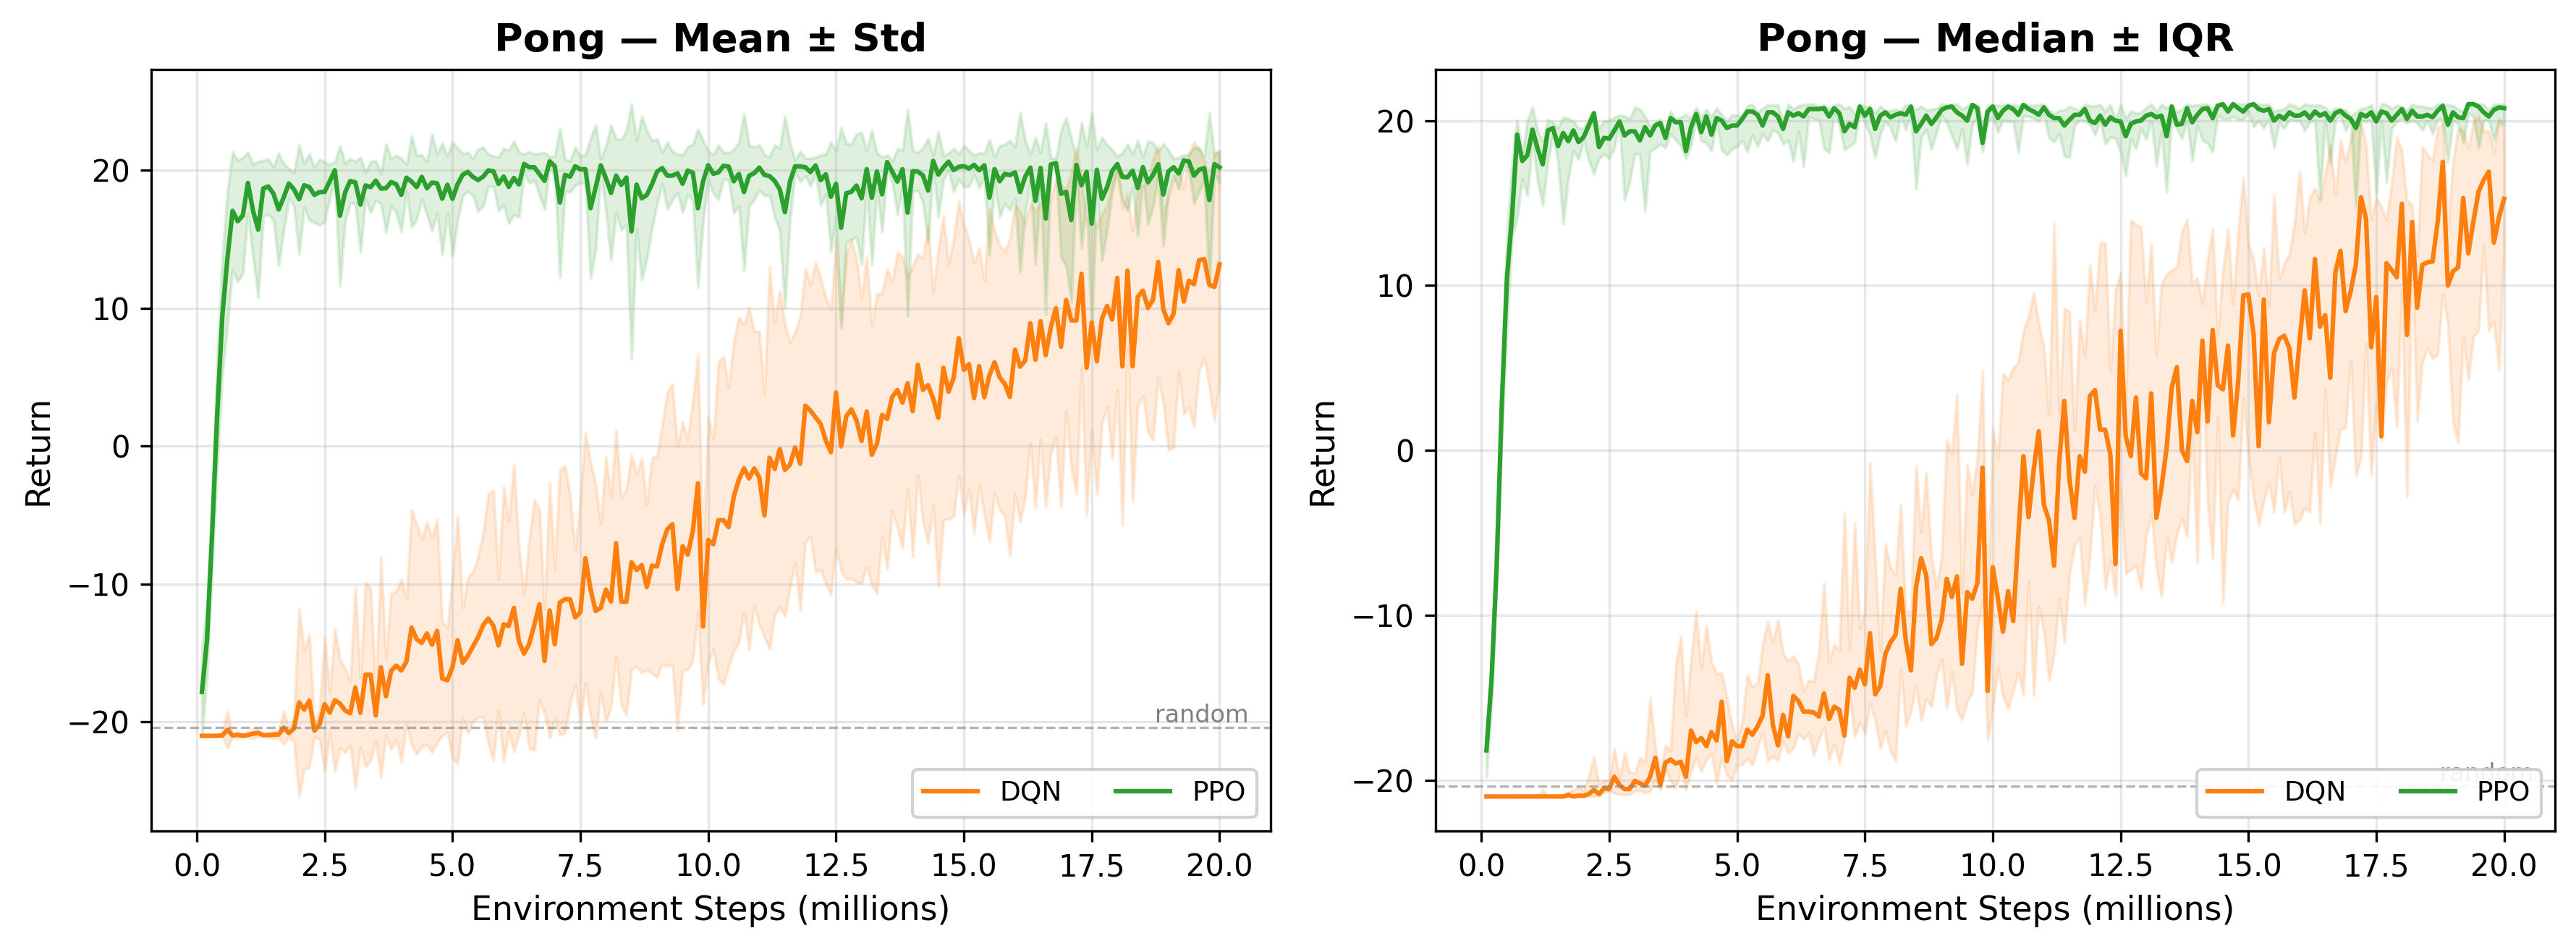
\includegraphics[width=\linewidth]{5_exp2_atari/assets/learning_curves_pong.png}
  \caption[Learning curves: Pong (DQN vs PPO)]{Learning curves for Pong. PPO converges near the maximum
           return of 21 within 3M steps; DQN shows high variance and
           most seeds remain negative.}
  \label{fig:atari-lc-pong}
\end{figure}

\subsection{Breakout}
\label{sec:breakout}

The surprise was that DQN outperformed PPO on Breakout.
DQN achieved a mean raw return of $43.62$ versus PPO's $32.51$, with
normalised IQM $0.100$ $[0.080,\;0.131]$ for DQN and $0.078$
$[0.062,\;0.095]$ for PPO. However, both algorithms achieve less than
11\% of the maximum return ($400$)---Breakout is far from solved.

DQN's best seed reaches $86.10$ (worst: $21.12$, IQR $16.15$),
while PPO's best seed is $47.04$ (worst: $19.64$, IQR $11.74$).
DQN's experience replay buffer likely provides an advantage here:
it can revisit rare brick-breaking trajectories that an on-policy
method like PPO discards after each update.
Figure~\ref{fig:atari-lc-breakout} shows the learning curves.

\begin{figure}[htbp!]
  \centering
  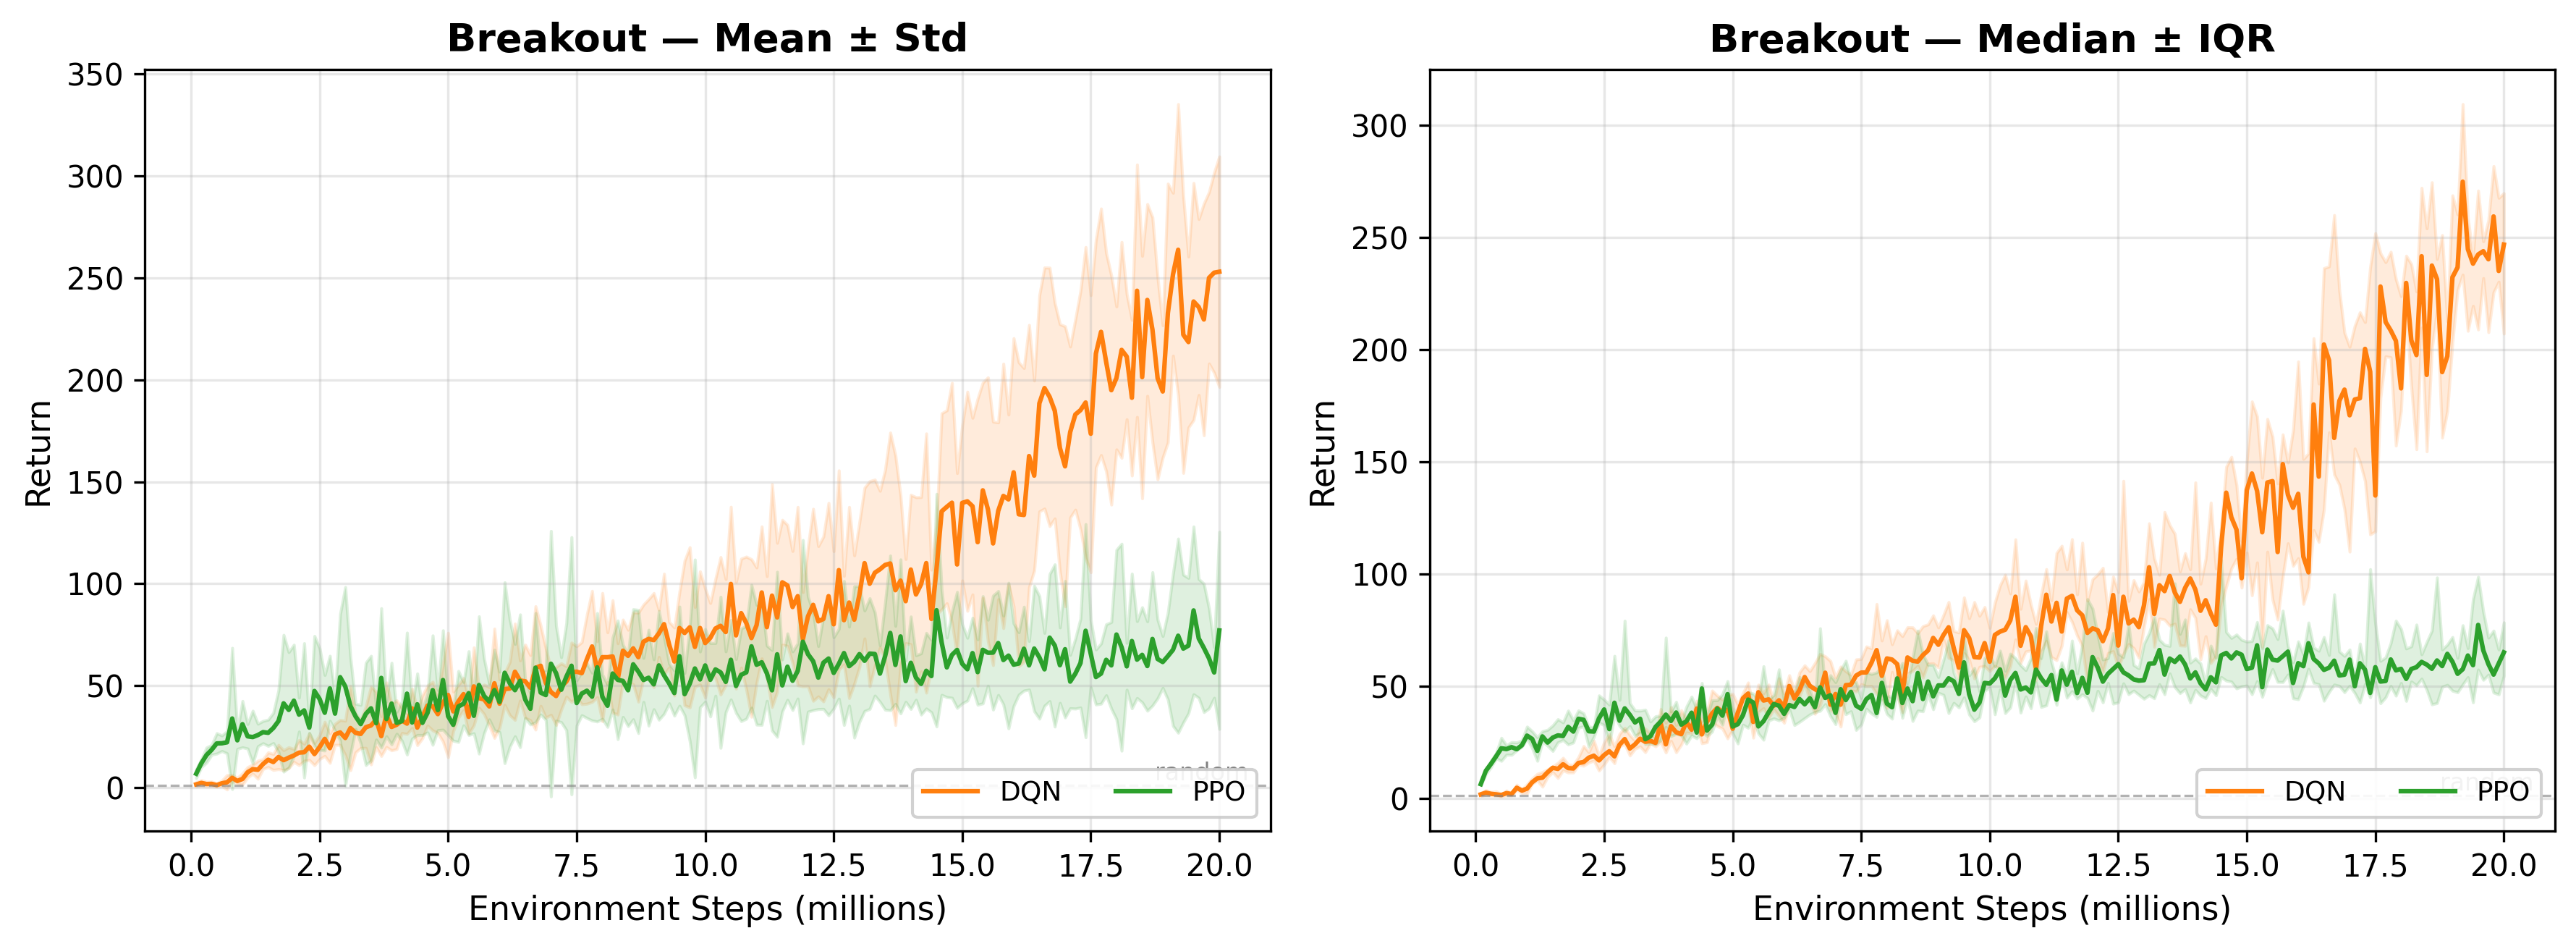
\includegraphics[width=\linewidth]{5_exp2_atari/assets/learning_curves_breakout.png}
  \caption[Learning curves: Breakout (DQN vs PPO)]{Learning curves for Breakout. DQN slightly outperforms PPO,
           but both remain below 11\% of the maximum score.}
  \label{fig:atari-lc-breakout}
\end{figure}

\subsection{Combined Learning Curves}
\label{sec:atari-combined-lc}

Figure~\ref{fig:atari-lc-combined} overlays both environments on a
normalised $y$-axis. PPO's Pong dominance is immediately visible as
a steep rise to near $1.0$; the Breakout curves for both algorithms
remain compressed near the bottom of the scale, with DQN slightly
ahead.

\begin{figure}[htbp!]
  \centering
  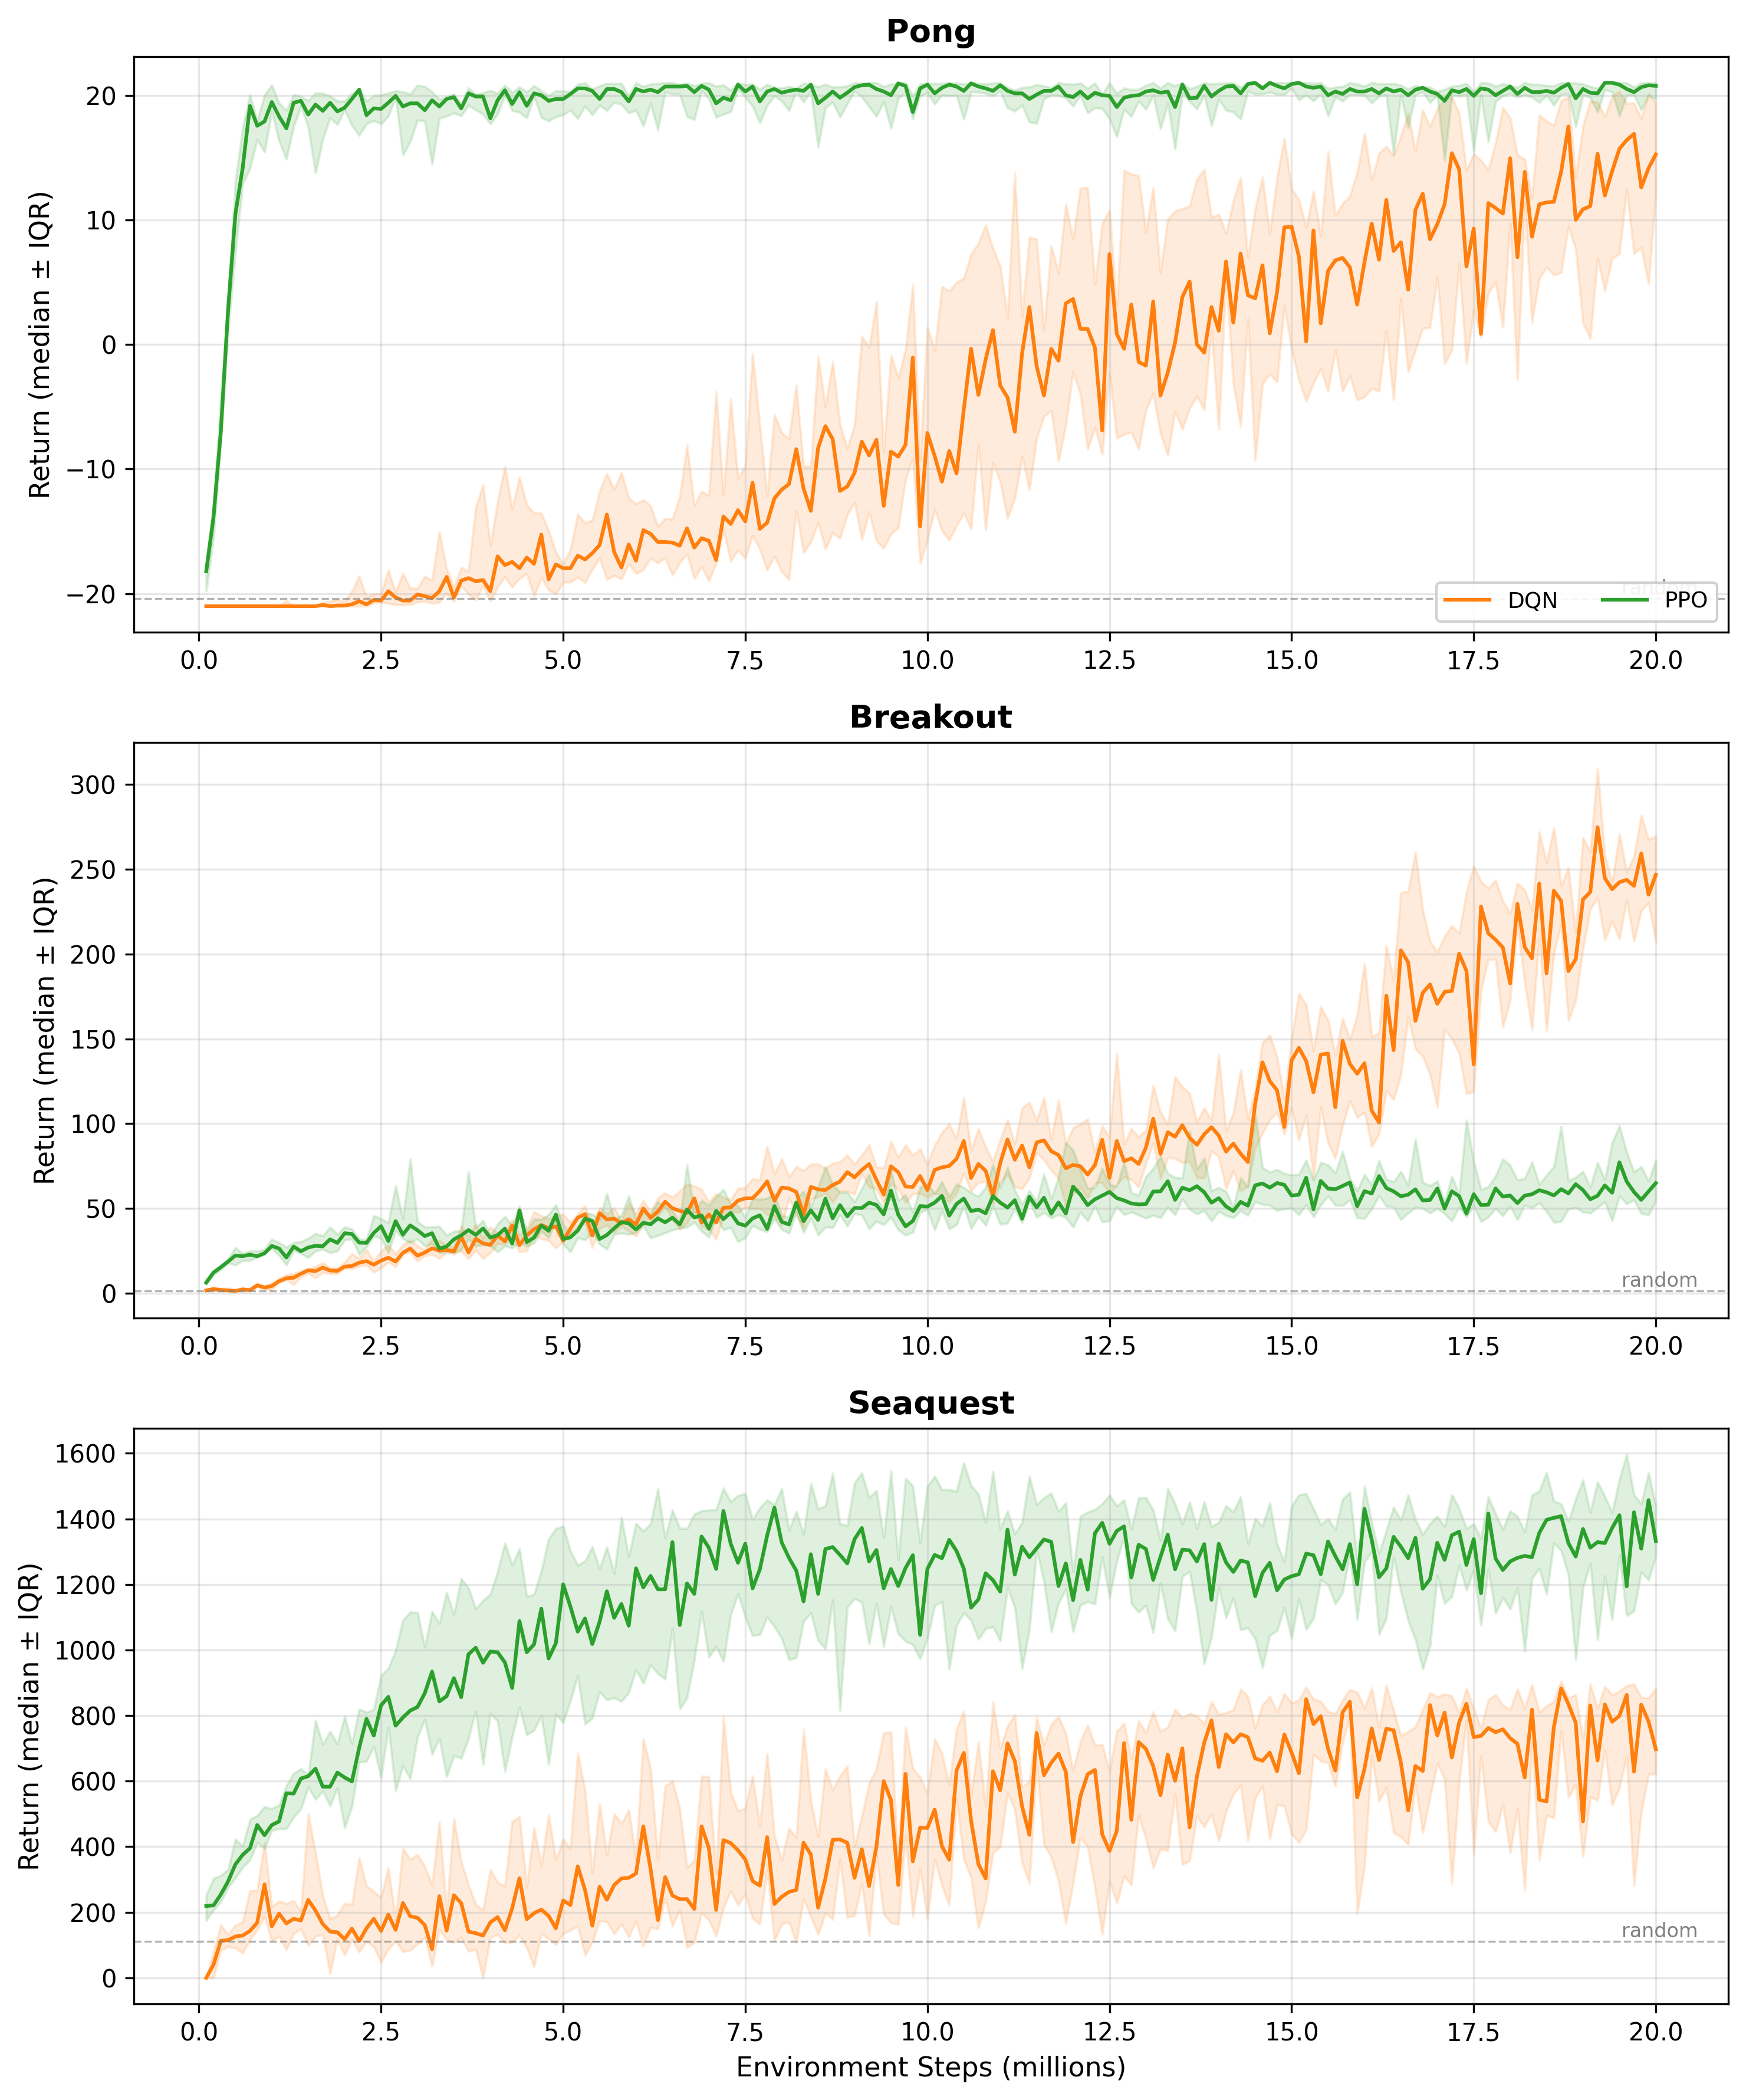
\includegraphics[width=\linewidth]{5_exp2_atari/assets/combined_learning_curves.png}
  \caption[Combined learning curves: Pong and Breakout]{Combined normalised learning curves for Pong and Breakout.
           PPO's Pong performance dominates the vertical scale.}
  \label{fig:atari-lc-combined}
\end{figure}

\subsection{Score Distributions and Per-Seed Analysis}
\label{sec:atari-score-dist}

Figures~\ref{fig:atari-score-dist},~\ref{fig:atari-heatmap},
and~\ref{fig:atari-boxswarm} provide three complementary views of the
per-seed results. The score distribution
(Figure~\ref{fig:atari-score-dist}) shows PPO's Pong scores
concentrated near $1.0$ while all Breakout scores cluster near zero.
The heatmap (Figure~\ref{fig:atari-heatmap}) makes this stark: the
PPO$\times$Pong column is uniformly green ($0.93$--$1.00$), while
the Breakout column is uniformly red for both algorithms. The
box-and-swarm plot (Figure~\ref{fig:atari-boxswarm}) highlights DQN's
wide spread on both environments.

\begin{figure}[htbp!]
  \centering
  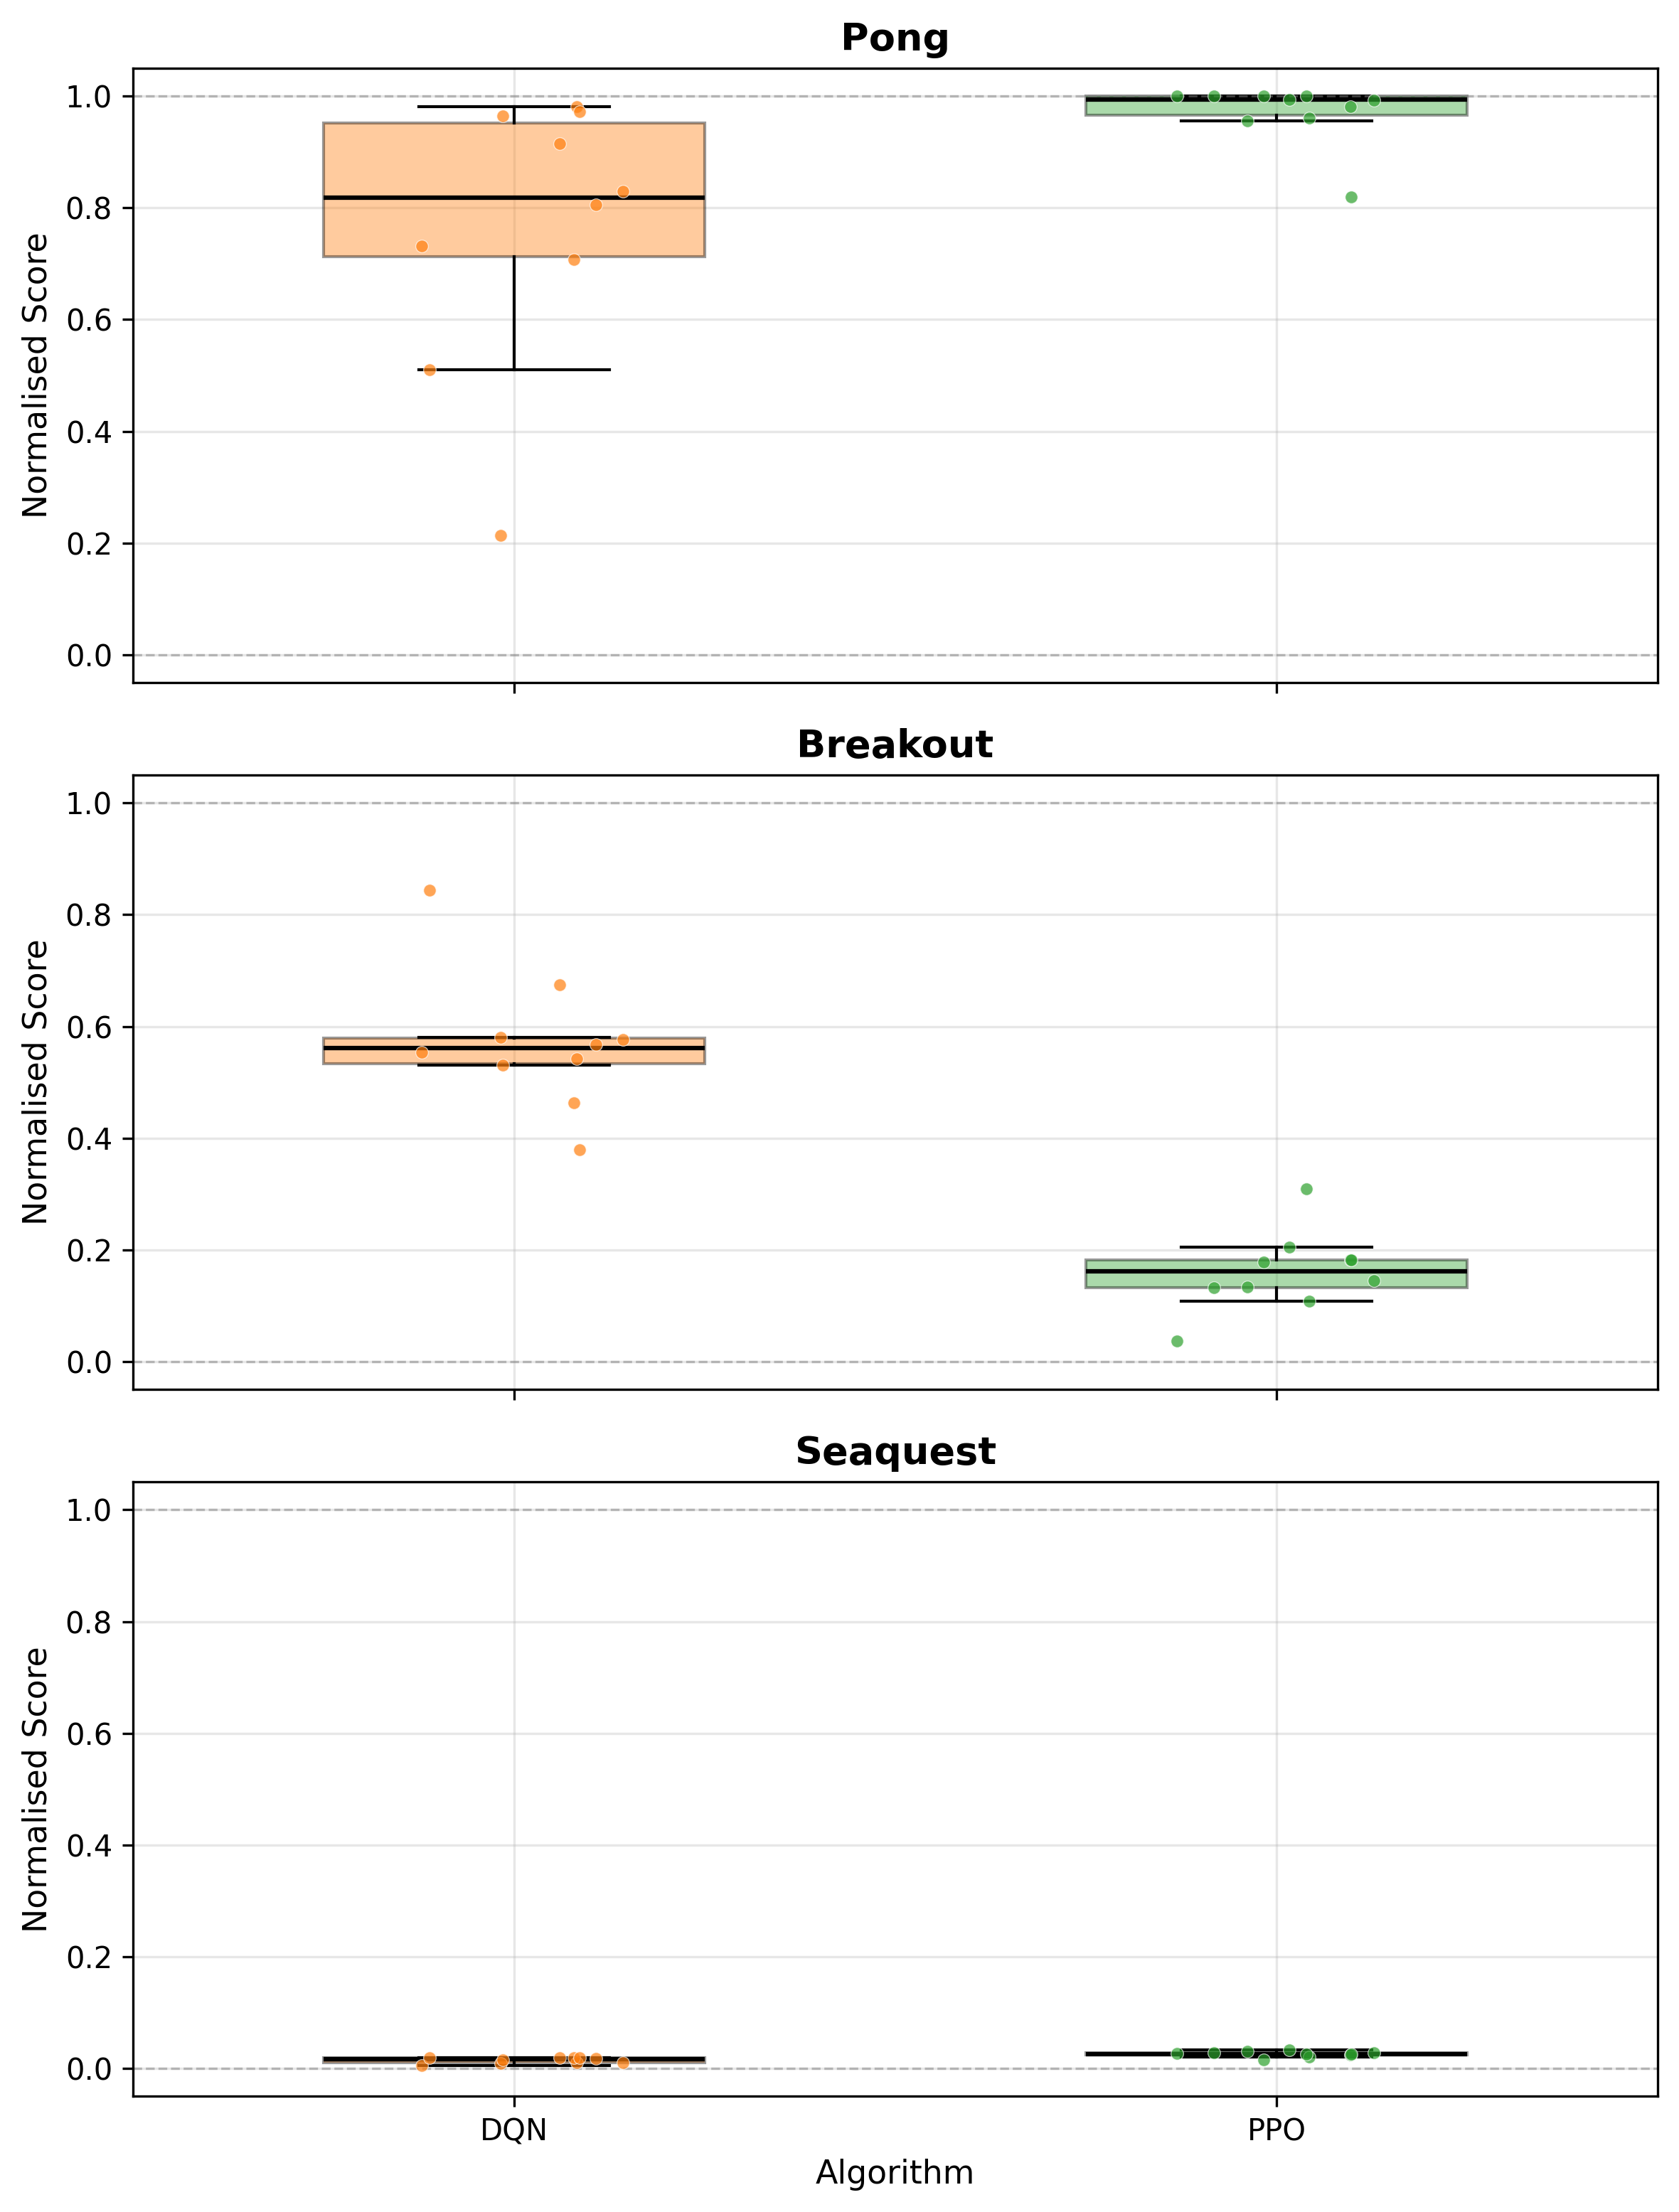
\includegraphics[width=\linewidth]{5_exp2_atari/assets/score_distribution.png}
  \caption[Score distributions: Pong and Breakout]{Distribution of normalised scores per environment. PPO Pong
           scores are concentrated near 1.0; all Breakout scores
           cluster near zero.}
  \label{fig:atari-score-dist}
\end{figure}

\begin{figure}[htbp!]
  \centering
  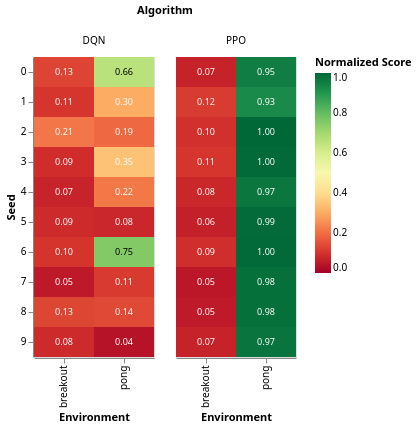
\includegraphics[width=\linewidth]{5_exp2_atari/assets/per_seed_heatmap.png}
  \caption[Per-seed score heatmap: Pong and Breakout]{Heatmap of normalised final scores by seed and environment.
           PPO$\times$Pong is uniformly high; Breakout performance is
           low for both algorithms.}
  \label{fig:atari-heatmap}
\end{figure}

\begin{figure}[htbp!]
  \centering
  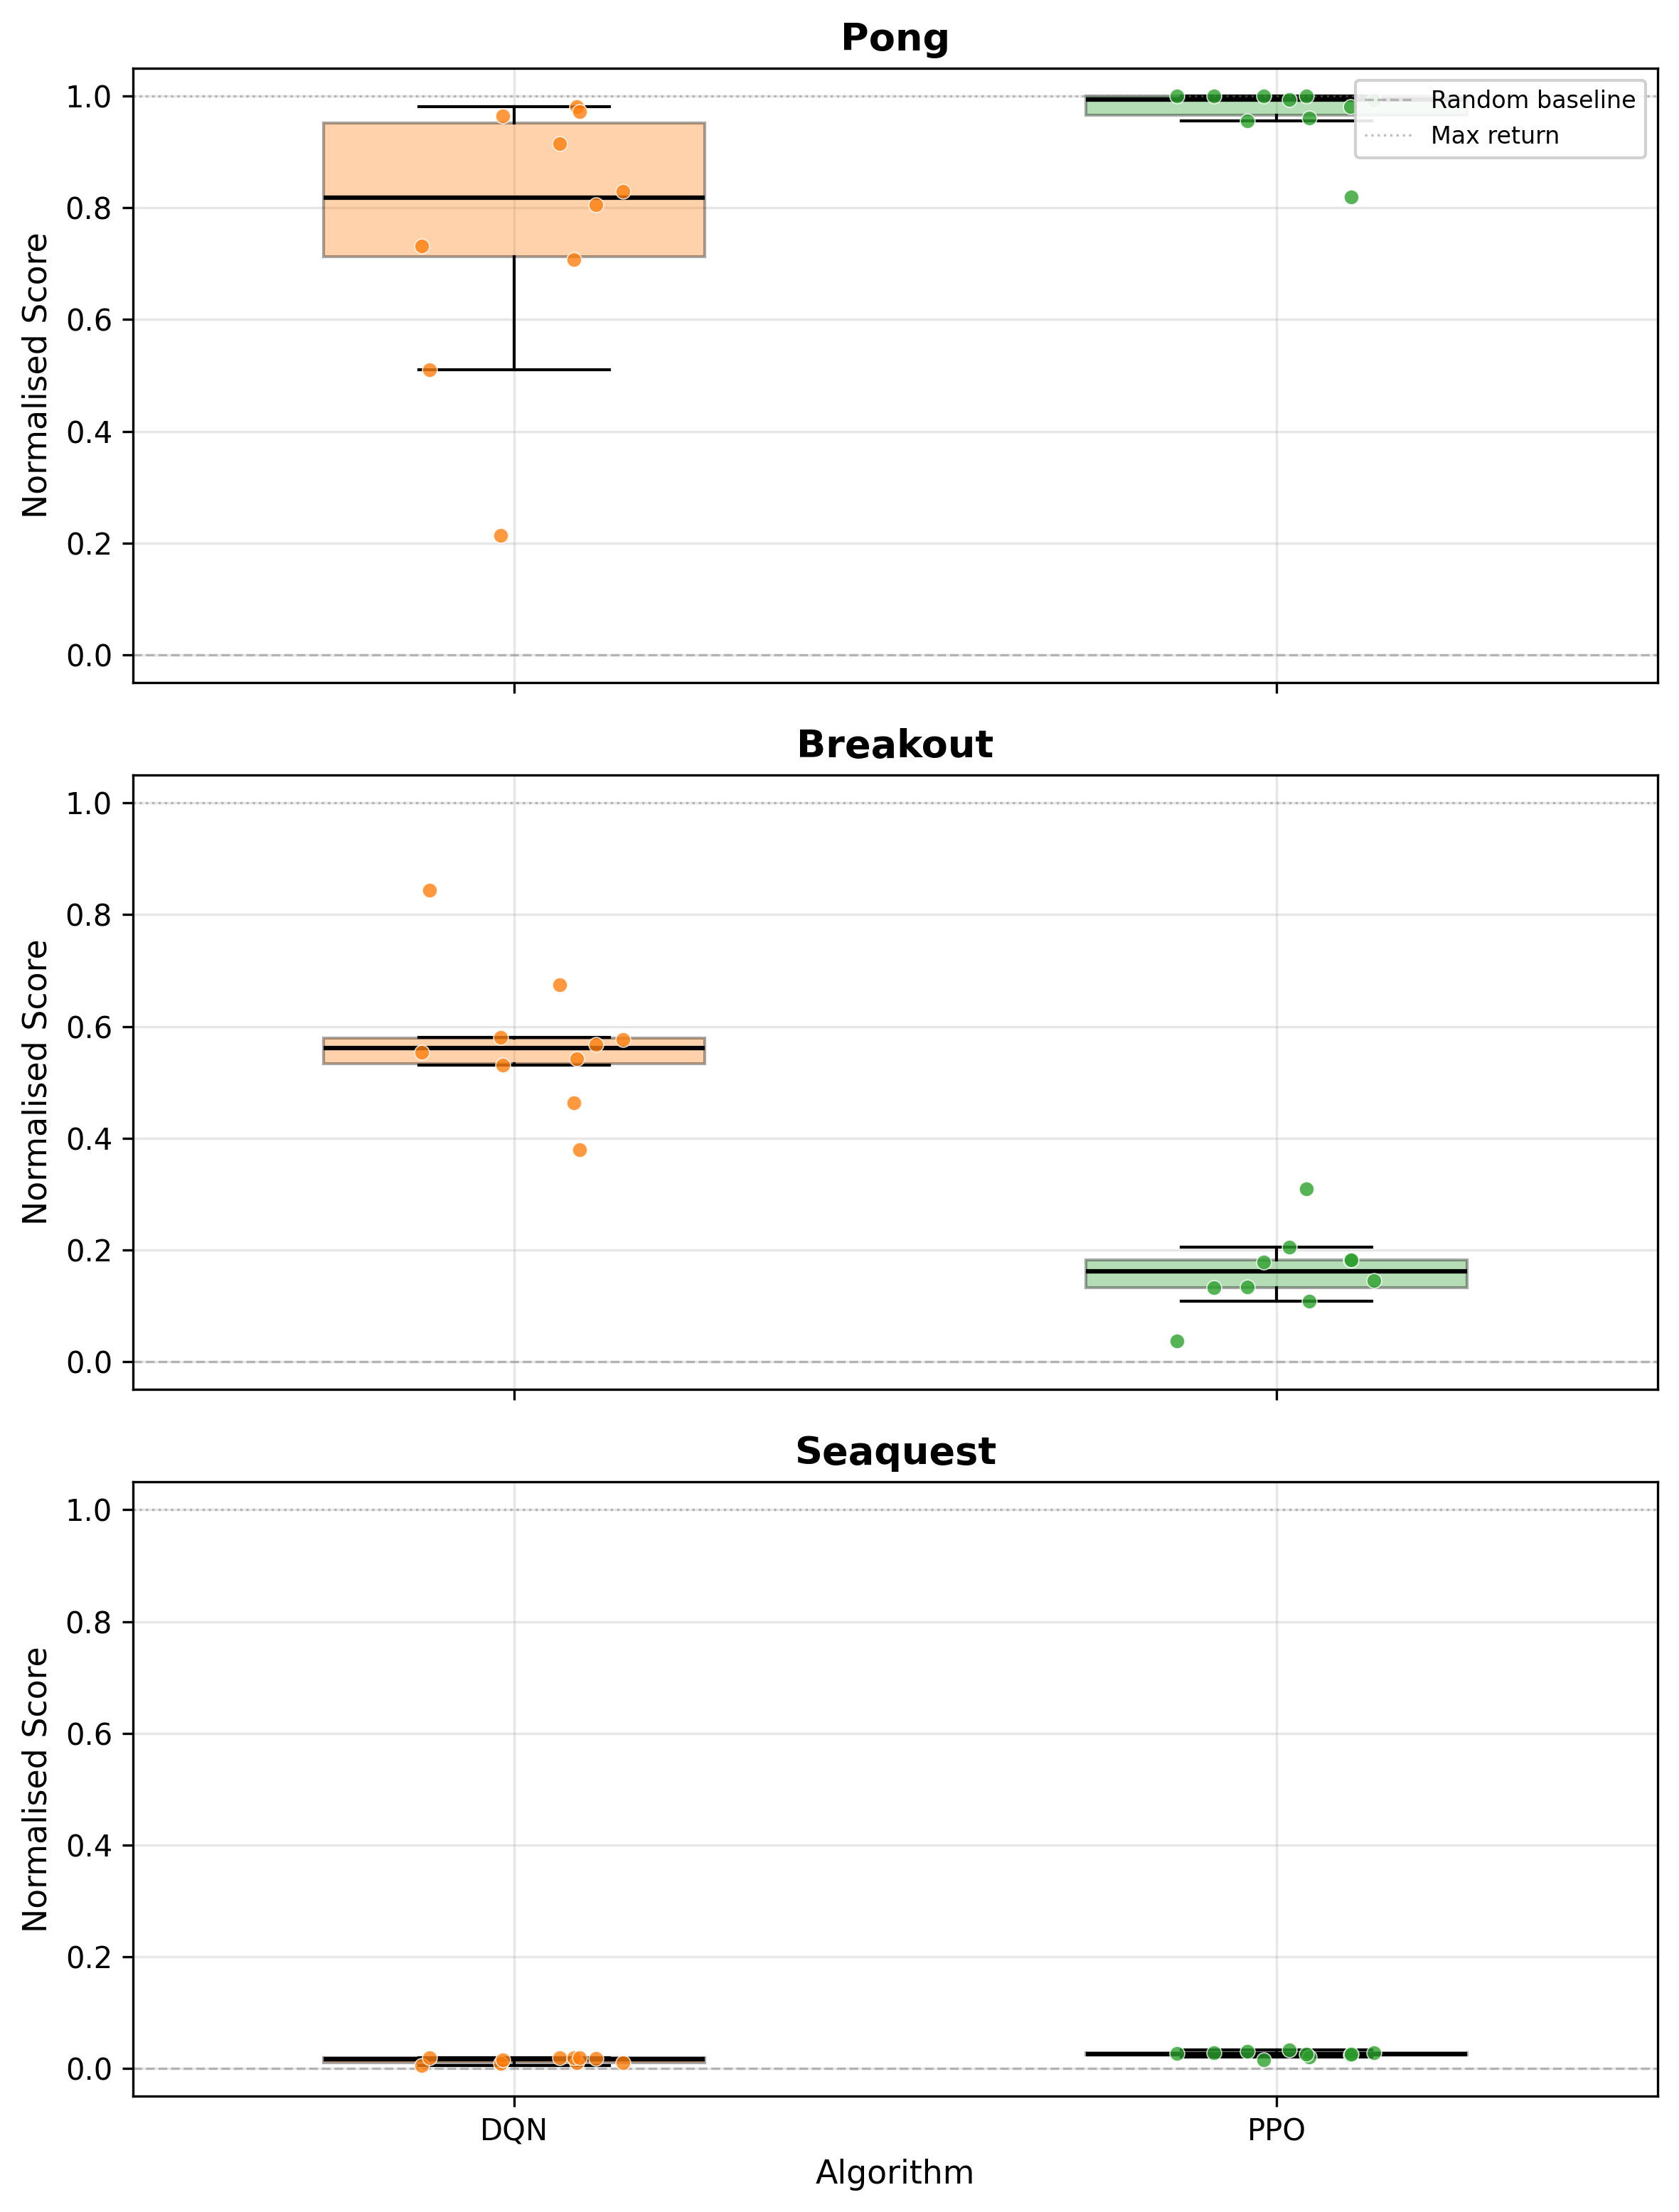
\includegraphics[width=\linewidth]{5_exp2_atari/assets/per_seed_boxswarm.png}
  \caption[Per-seed score spread: Pong and Breakout]{Box-and-swarm plot of per-seed normalised scores. DQN
           exhibits the widest spread on both environments.}
  \label{fig:atari-boxswarm}
\end{figure}

Table~\ref{tab:atari-per-env-iqm} summarises the per-environment
normalised IQM with 95\% bootstrap confidence intervals.

\begin{table}[htbp!]
\centering
\caption{Per-environment normalised IQM with 95\% bootstrap CIs.}
\label{tab:atari-per-env-iqm}
\begin{tabular}{lcc}
\toprule
\textbf{Algorithm} & \textbf{Pong} & \textbf{Breakout} \\
\midrule
PPO & $0.983\;[0.963,\;0.993]$ & $0.078\;[0.062,\;0.095]$ \\
DQN & $0.217\;[0.121,\;0.445]$ & $0.100\;[0.080,\;0.131]$ \\
\bottomrule
\end{tabular}
\end{table}

%% ------------------------------------------------------------------
\section{Cross-Environment Aggregate Results}
\label{sec:atari-cross-env}

\subsection{Final Performance}
\label{sec:atari-final-perf}

Table~\ref{tab:atari-cross-env} reports the cross-environment aggregate
metrics at the final training budget. PPO achieves a higher IQM
($0.529$) than DQN ($0.130$), but this is heavily driven by PPO's
near-perfect Pong performance. Both optimality gaps are large.

\begin{table}[htbp!]
\centering
\caption{Cross-environment aggregate metrics (normalised scores). IQM,
         mean, and median are reported with 95\% bootstrap CIs.}
\label{tab:atari-cross-env}
\resizebox{\linewidth}{!}{%
\begin{tabular}{lcccc}
\toprule
\textbf{Algorithm} & \textbf{IQM} & \textbf{Mean} & \textbf{Median}
                   & \textbf{Opt.\ Gap} \\
\midrule
PPO & $0.529\;[0.514,\;0.542]$ & $0.528\;[0.518,\;0.537]$
    & $0.528\;[0.518,\;0.537]$
    & $0.472\;[0.463,\;0.482]$ \\
DQN & $0.130\;[0.098,\;0.184]$ & $0.195\;[0.129,\;0.272]$
    & $0.195\;[0.129,\;0.272]$
    & $0.805\;[0.728,\;0.872]$ \\
\bottomrule
\end{tabular}}
\end{table}

\begin{figure}[htbp!]
  \centering
  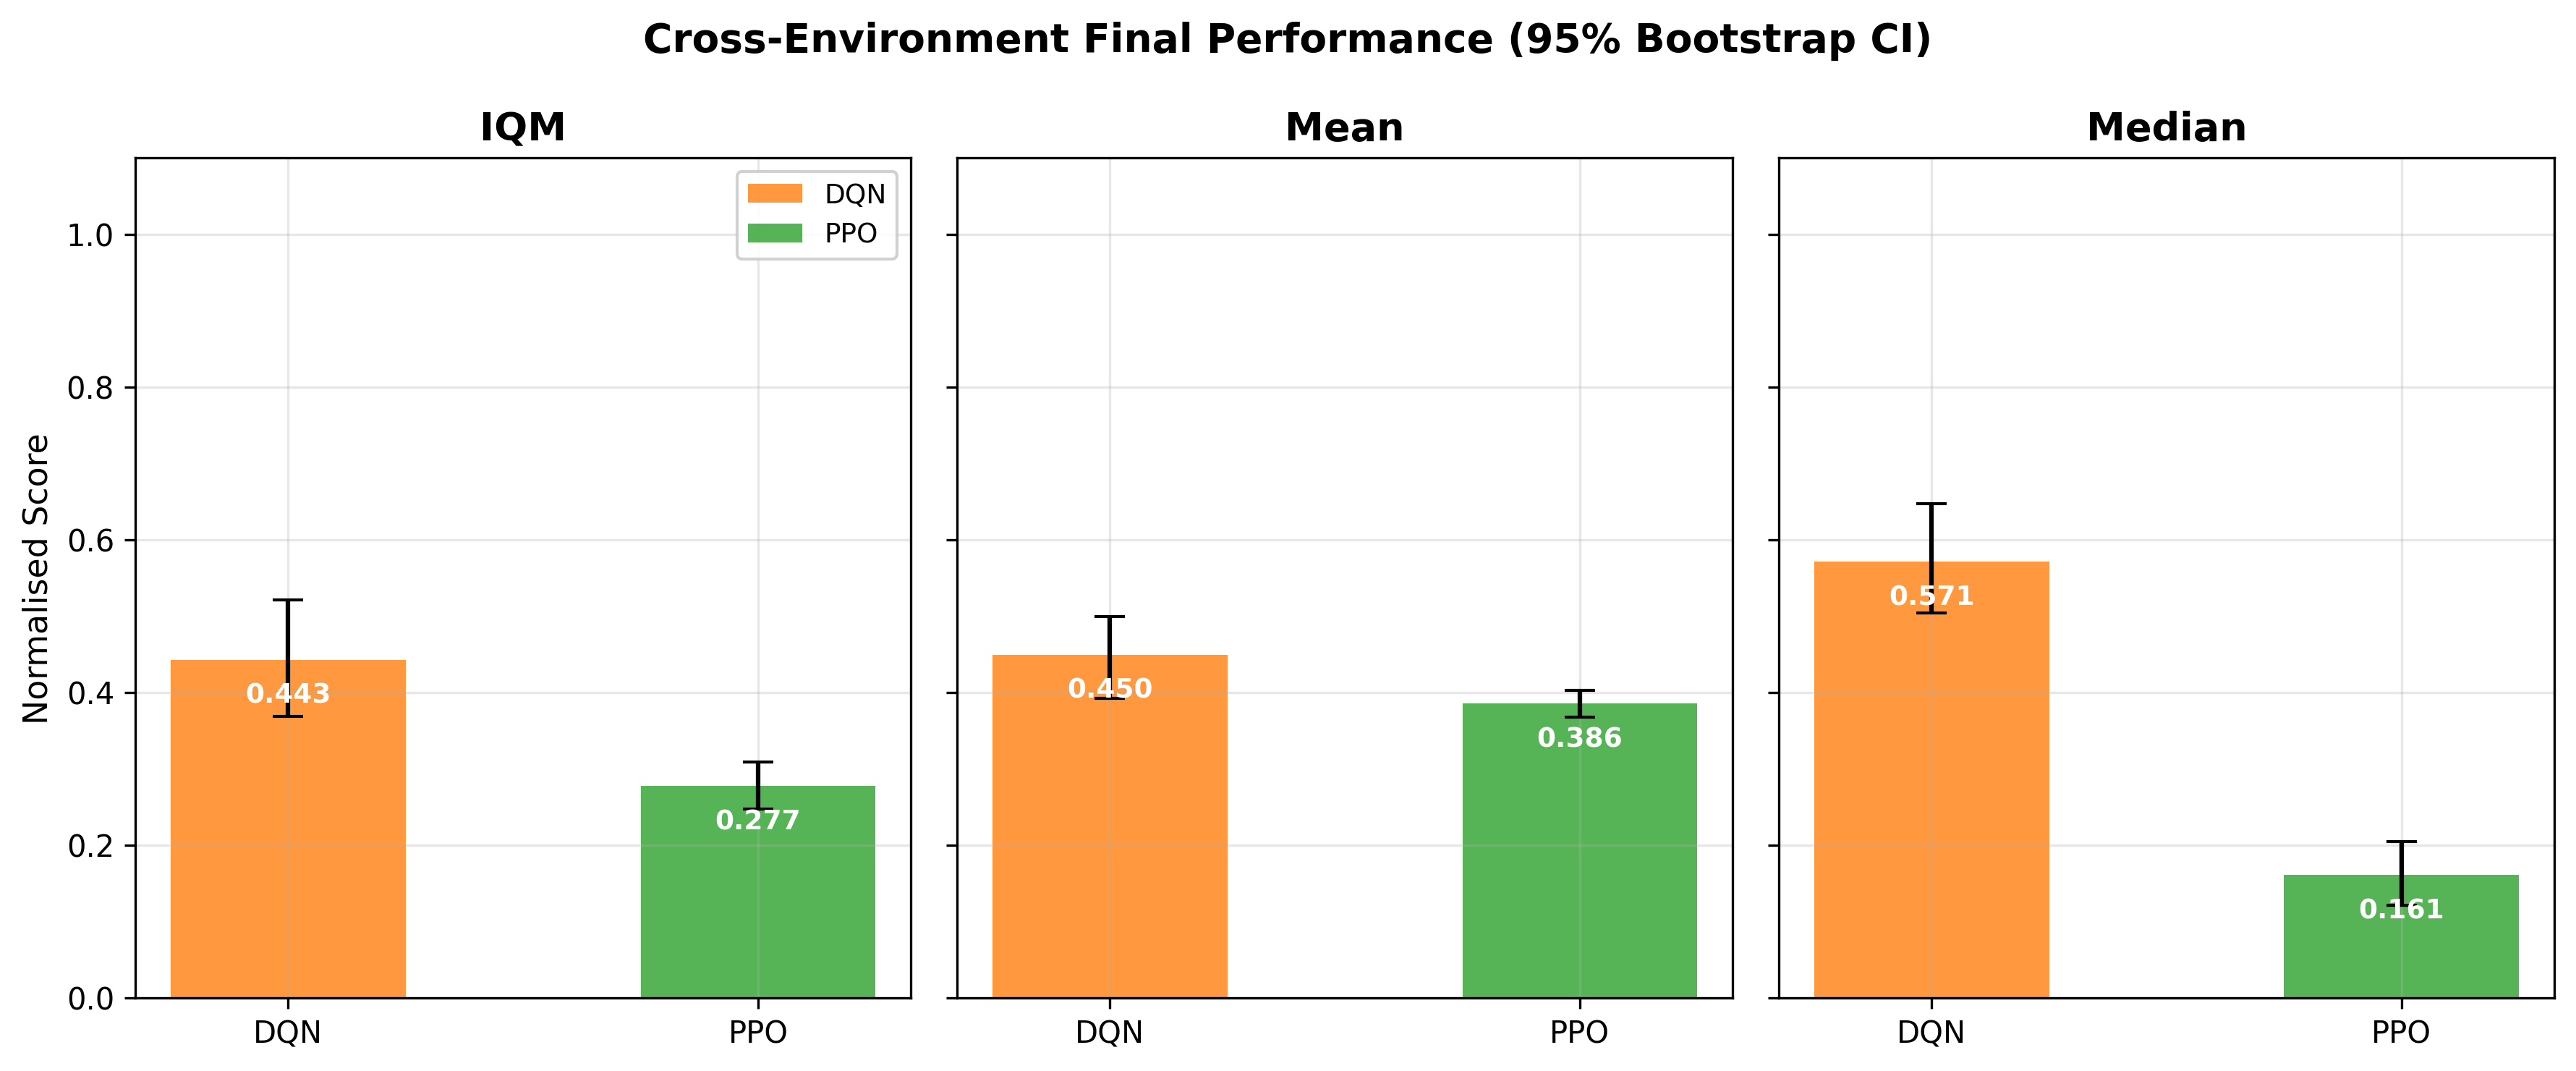
\includegraphics[width=\linewidth]{5_exp2_atari/assets/final_performance.png}
  \caption[Cross-environment IQM: Pong and Breakout]{Cross-environment IQM, mean, and median with 95\% bootstrap
           confidence intervals.}
  \label{fig:atari-final-perf}
\end{figure}

\subsection{Performance Profile and Optimality Gap}
\label{sec:atari-profile-gap}

The performance profile (Figure~\ref{fig:atari-perf-profile}) reveals
the bimodal nature of the score distributions. PPO maintains
$\hat{F}(\tau) = 0.50$ from $\tau = 0.12$ all the way to
$\tau = 0.92$: half its runs (the Pong seeds) score near $1.0$
while the other half (Breakout seeds) cluster near $0.08$, with
nothing in between. DQN drops below $0.50$ at $\tau = 0.12$.

\begin{figure}[htbp!]
  \centering
  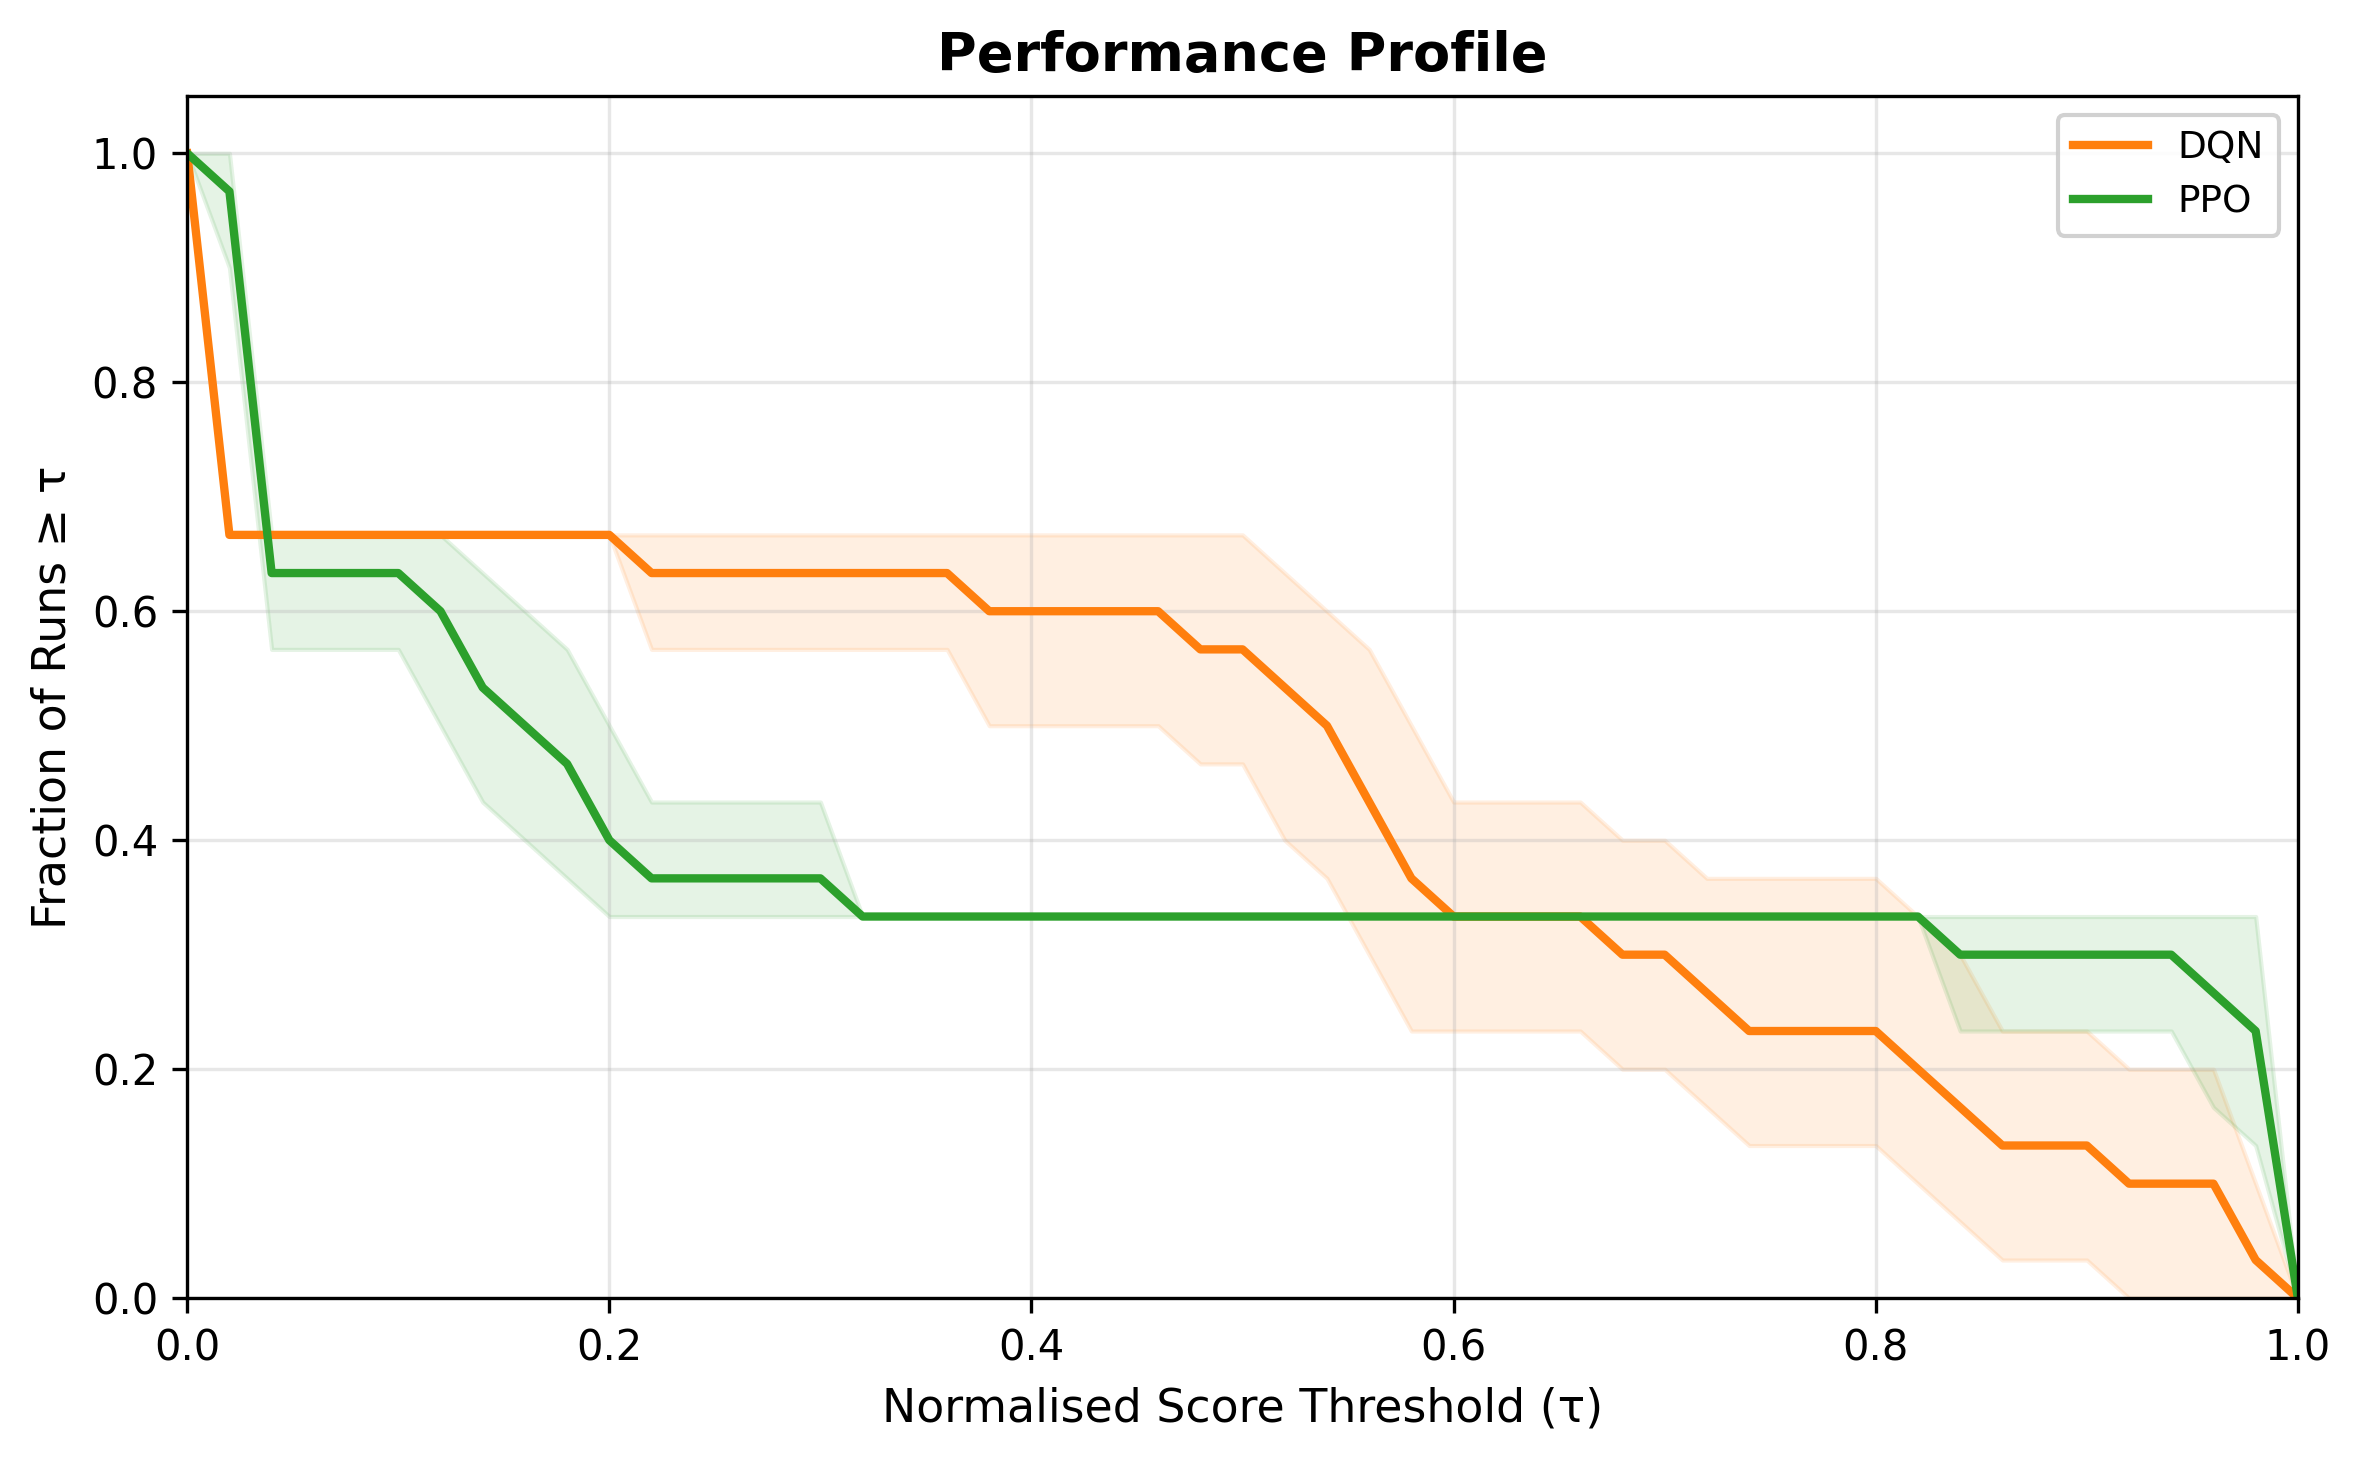
\includegraphics[width=\linewidth]{5_exp2_atari/assets/performance_profile.png}
  \caption[Performance profiles: Pong and Breakout]{Performance profiles with 95\% bootstrap CIs. PPO's flat
           plateau at 0.50 reflects its bimodal Pong/Breakout split.}
  \label{fig:atari-perf-profile}
\end{figure}

\begin{figure}[htbp!]
  \centering
  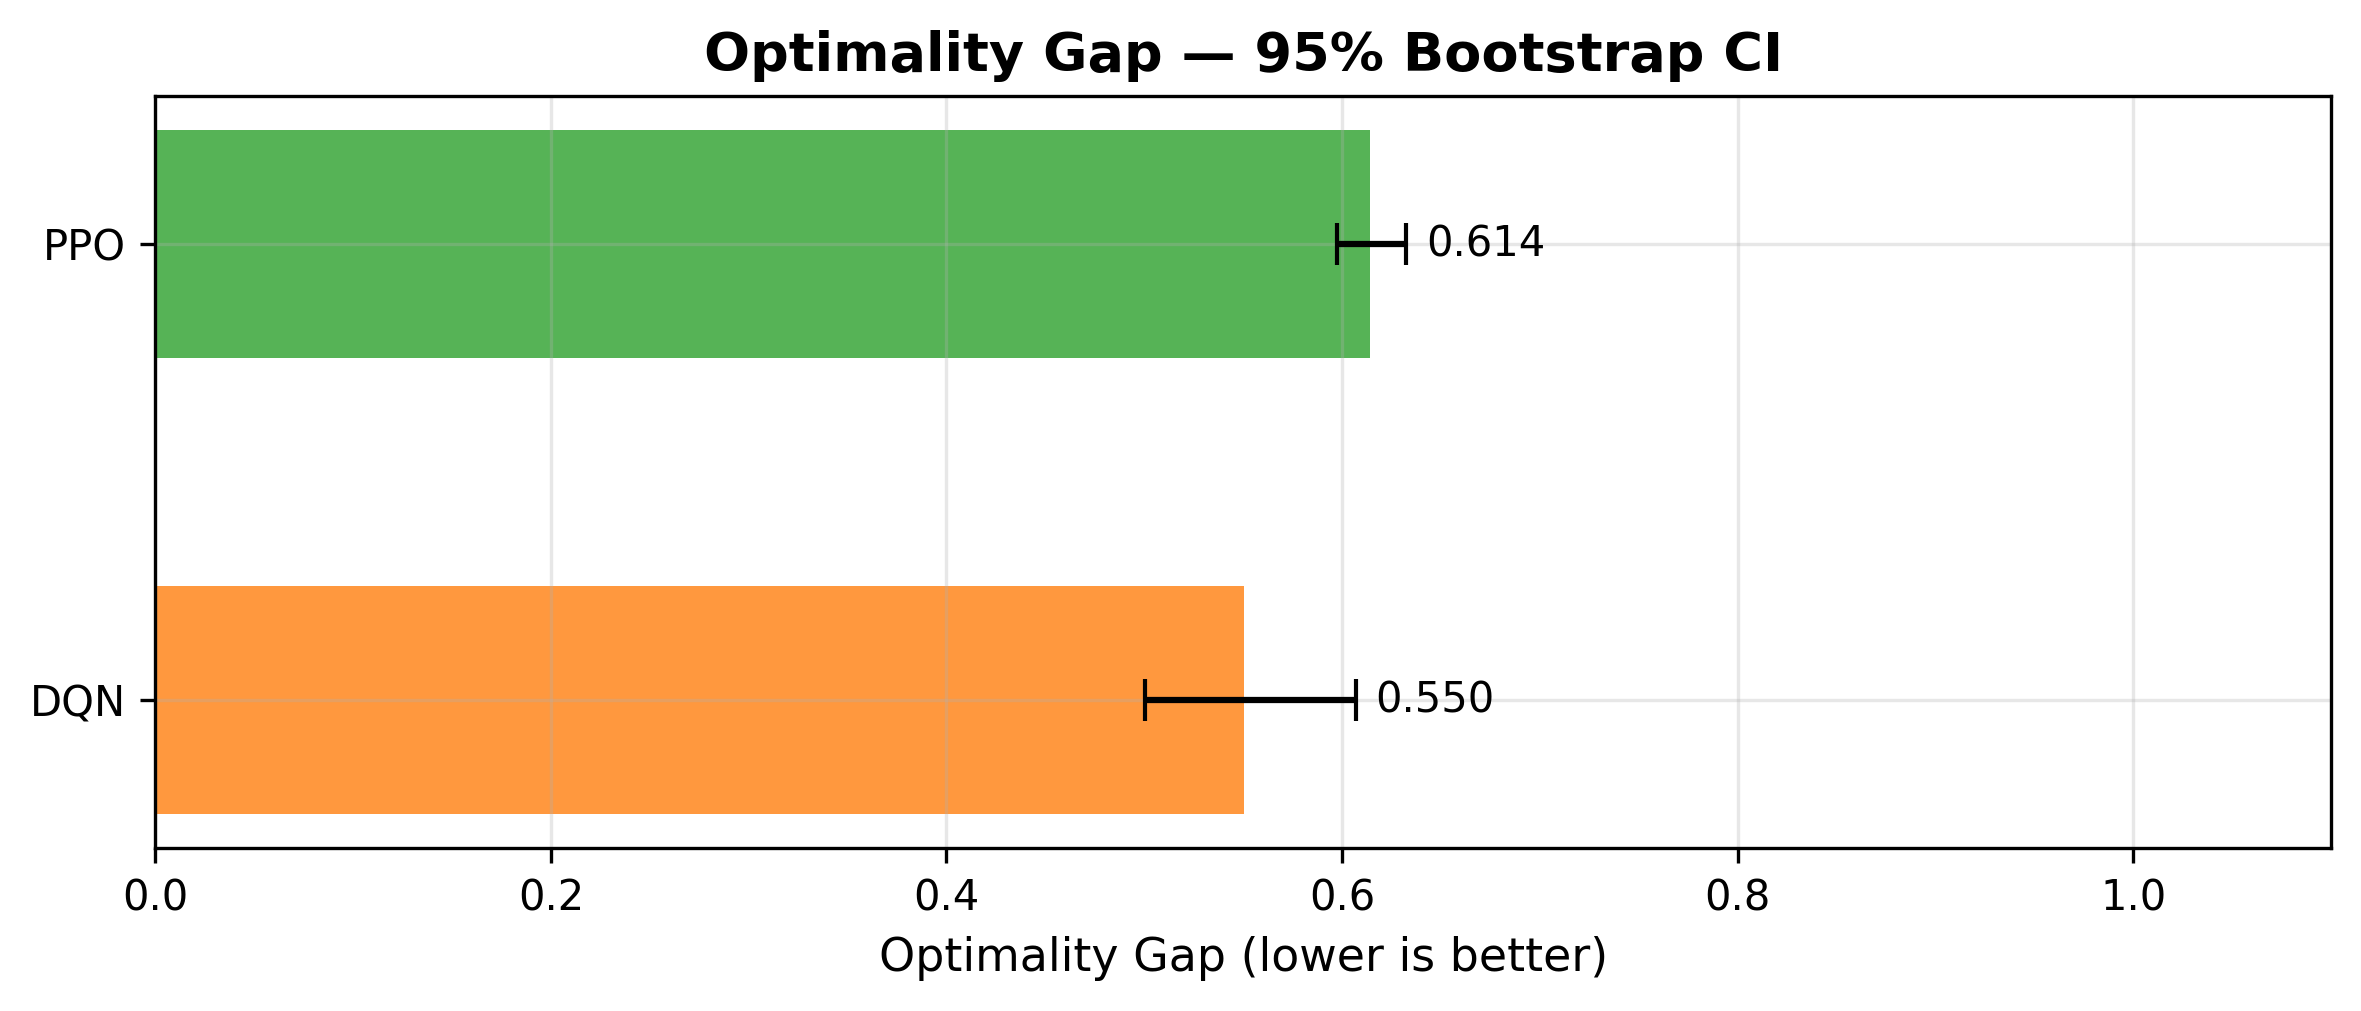
\includegraphics[width=\linewidth]{5_exp2_atari/assets/optimality_gap.png}
  \caption[Optimality gap: Pong and Breakout]{Optimality gap with 95\% bootstrap CIs. Both algorithms
           have large gaps: PPO $0.472$, DQN $0.805$.}
  \label{fig:atari-opt-gap}
\end{figure}

\subsection{Sample Efficiency}
\label{sec:atari-sample-eff}

\begin{figure}[htbp!]
  \centering
  \begin{subfigure}[b]{0.48\linewidth}
    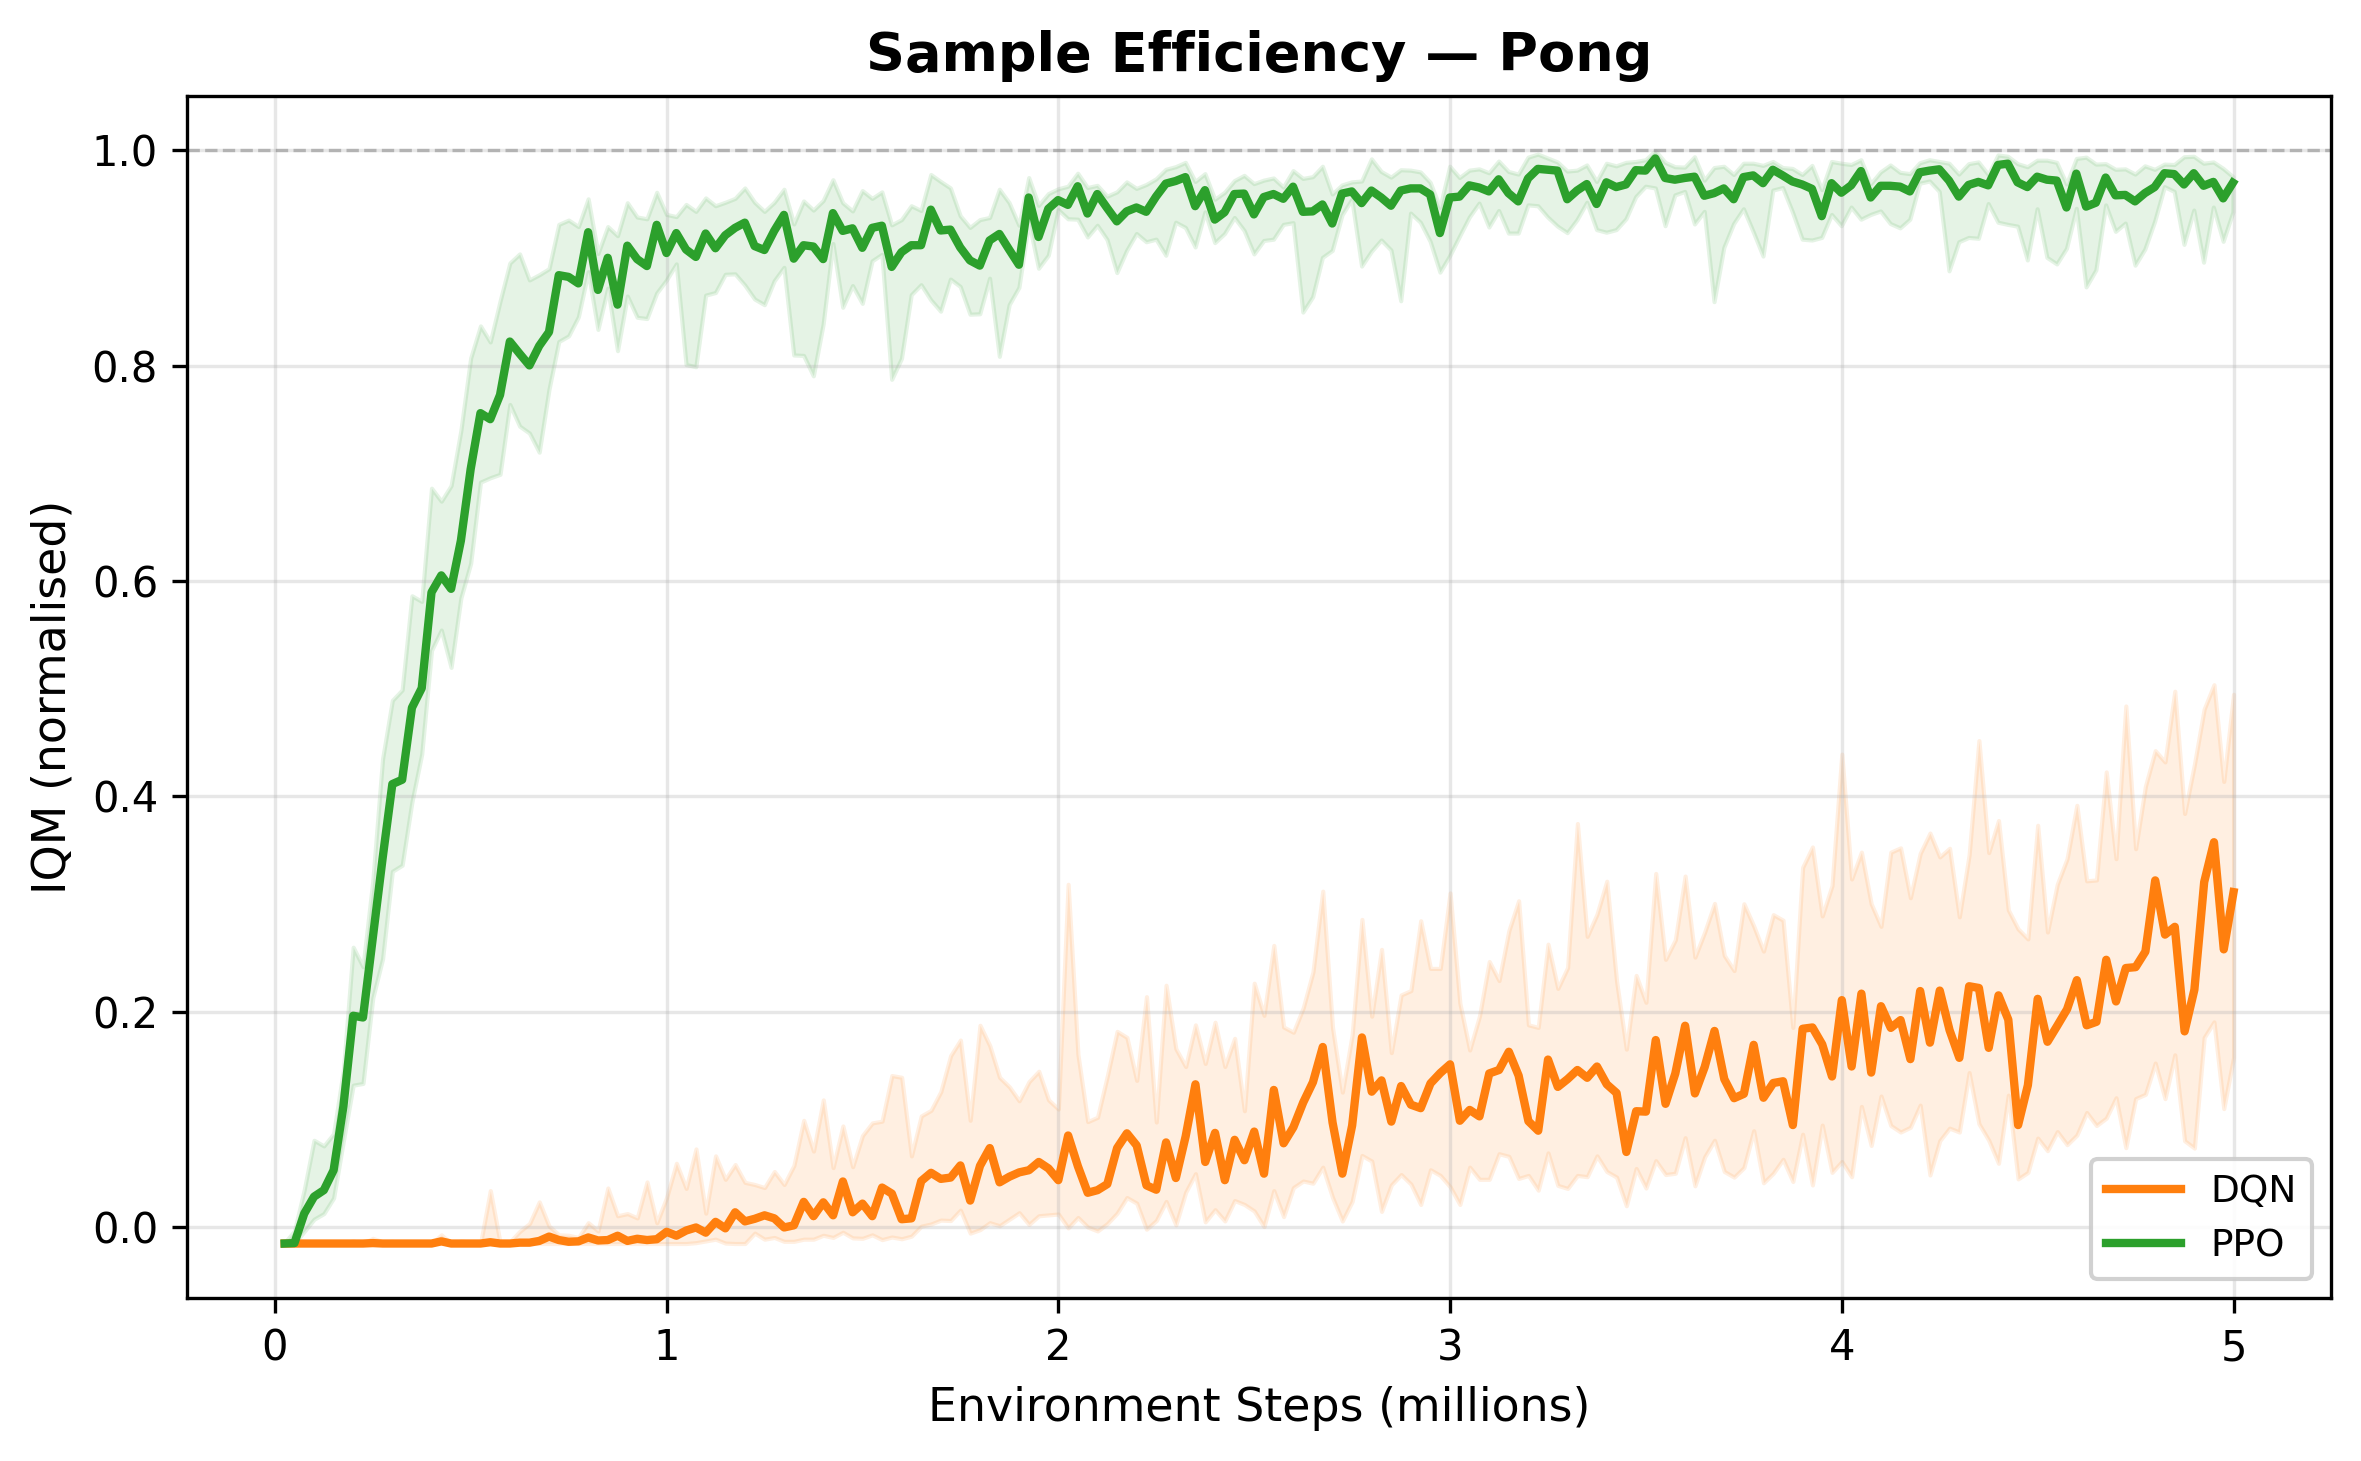
\includegraphics[width=\linewidth]{5_exp2_atari/assets/sample_efficiency_pong.png}
    \caption{Pong}
    \label{fig:atari-se-pong}
  \end{subfigure}
  \hfill
  \begin{subfigure}[b]{0.48\linewidth}
    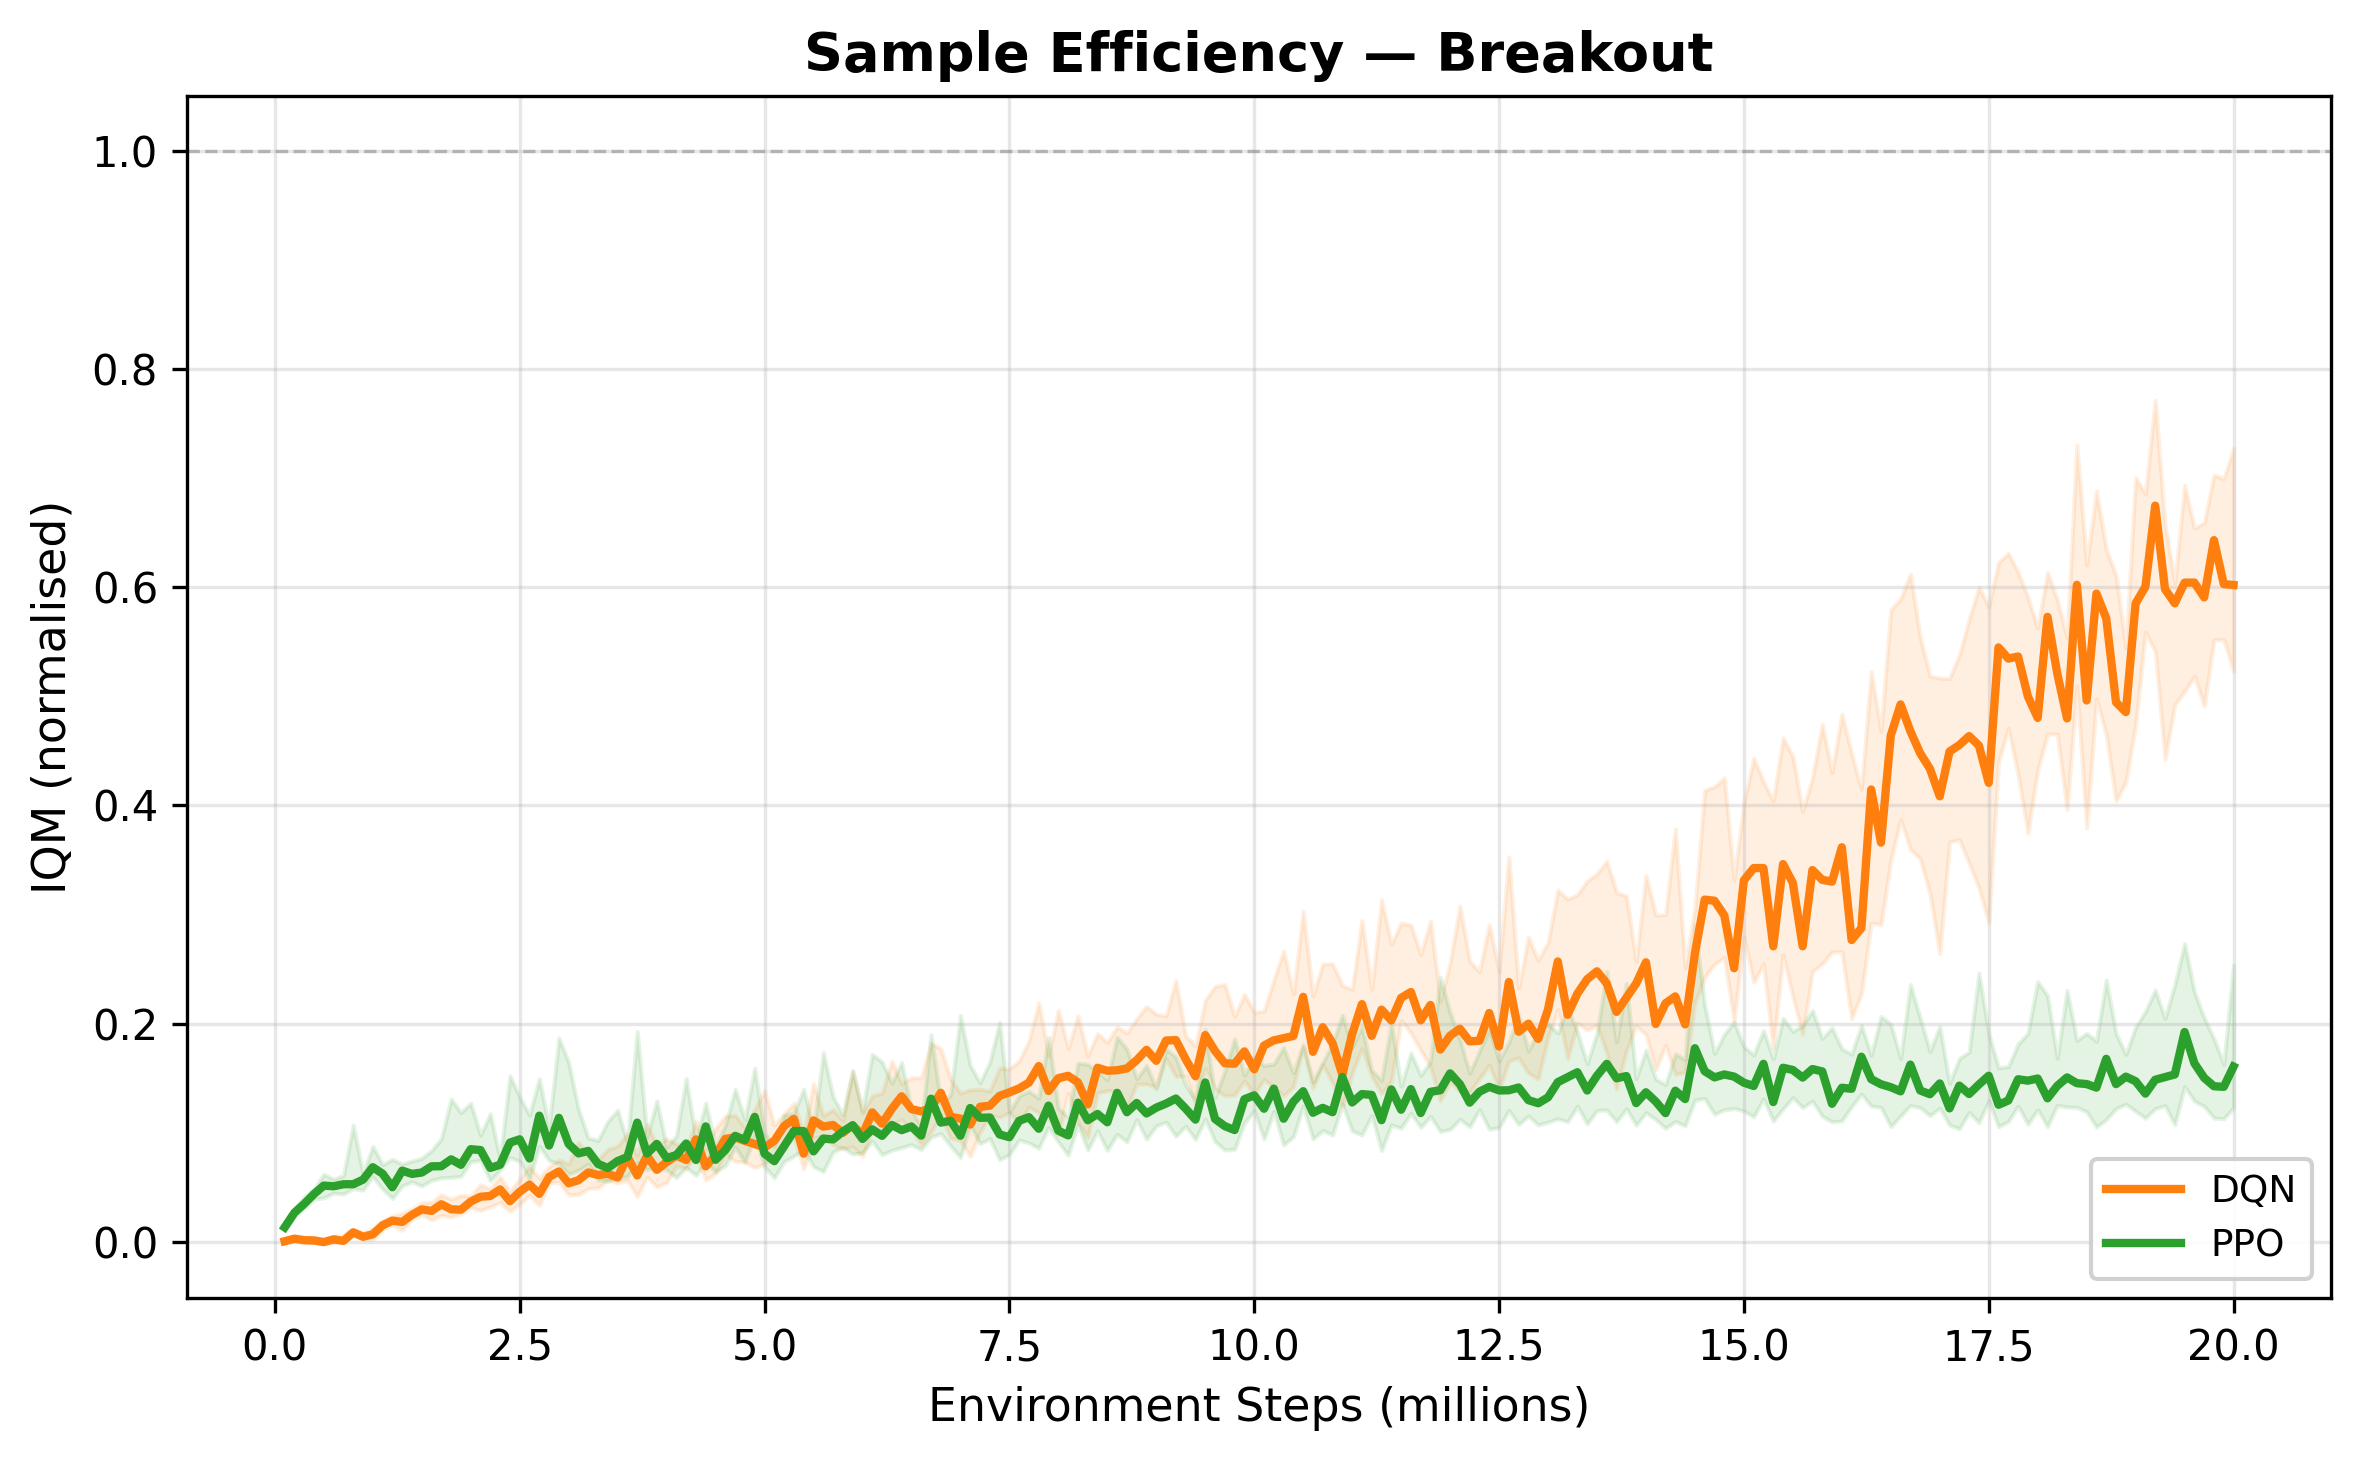
\includegraphics[width=\linewidth]{5_exp2_atari/assets/sample_efficiency_breakout.png}
    \caption{Breakout}
    \label{fig:atari-se-breakout}
  \end{subfigure}
  \caption[Sample efficiency: Pong and Breakout]{Sample efficiency (normalised AUC) per environment. PPO is
           dramatically more sample-efficient on Pong; on Breakout the
           difference is small.}
  \label{fig:atari-sample-eff}
\end{figure}

Table~\ref{tab:atari-sample-eff} reports the normalised AUC values.
On Pong, PPO's AUC ($0.876$) is nearly $10\times$ that of DQN
($0.090$), reflecting PPO's rapid convergence. On Breakout, the gap
is much smaller: PPO $0.070$ versus DQN $0.048$.

\begin{table}[htbp!]
\centering
\caption{Sample efficiency (normalised AUC) per environment.}
\label{tab:atari-sample-eff}
\begin{tabular}{lcc}
\toprule
\textbf{Algorithm} & \textbf{Pong} & \textbf{Breakout} \\
\midrule
PPO & 0.876 & 0.070 \\
DQN & 0.090 & 0.048 \\
\bottomrule
\end{tabular}
\end{table}

\subsection{Pairwise Probability of Improvement}
\label{sec:atari-poi}

Figure~\ref{fig:atari-poi} shows the pairwise probability of
improvement. $P(\text{DQN} > \text{PPO}) = 0.353$, so
$P(\text{PPO} > \text{DQN}) = 0.648$. This is notably less decisive
than Experiment~1, where PPO had $P > 0.89$ against all
competitors. DQN's Breakout advantage partially offsets its Pong
deficit, preventing a clear-cut verdict.

\begin{figure}[htbp!]
  \centering
  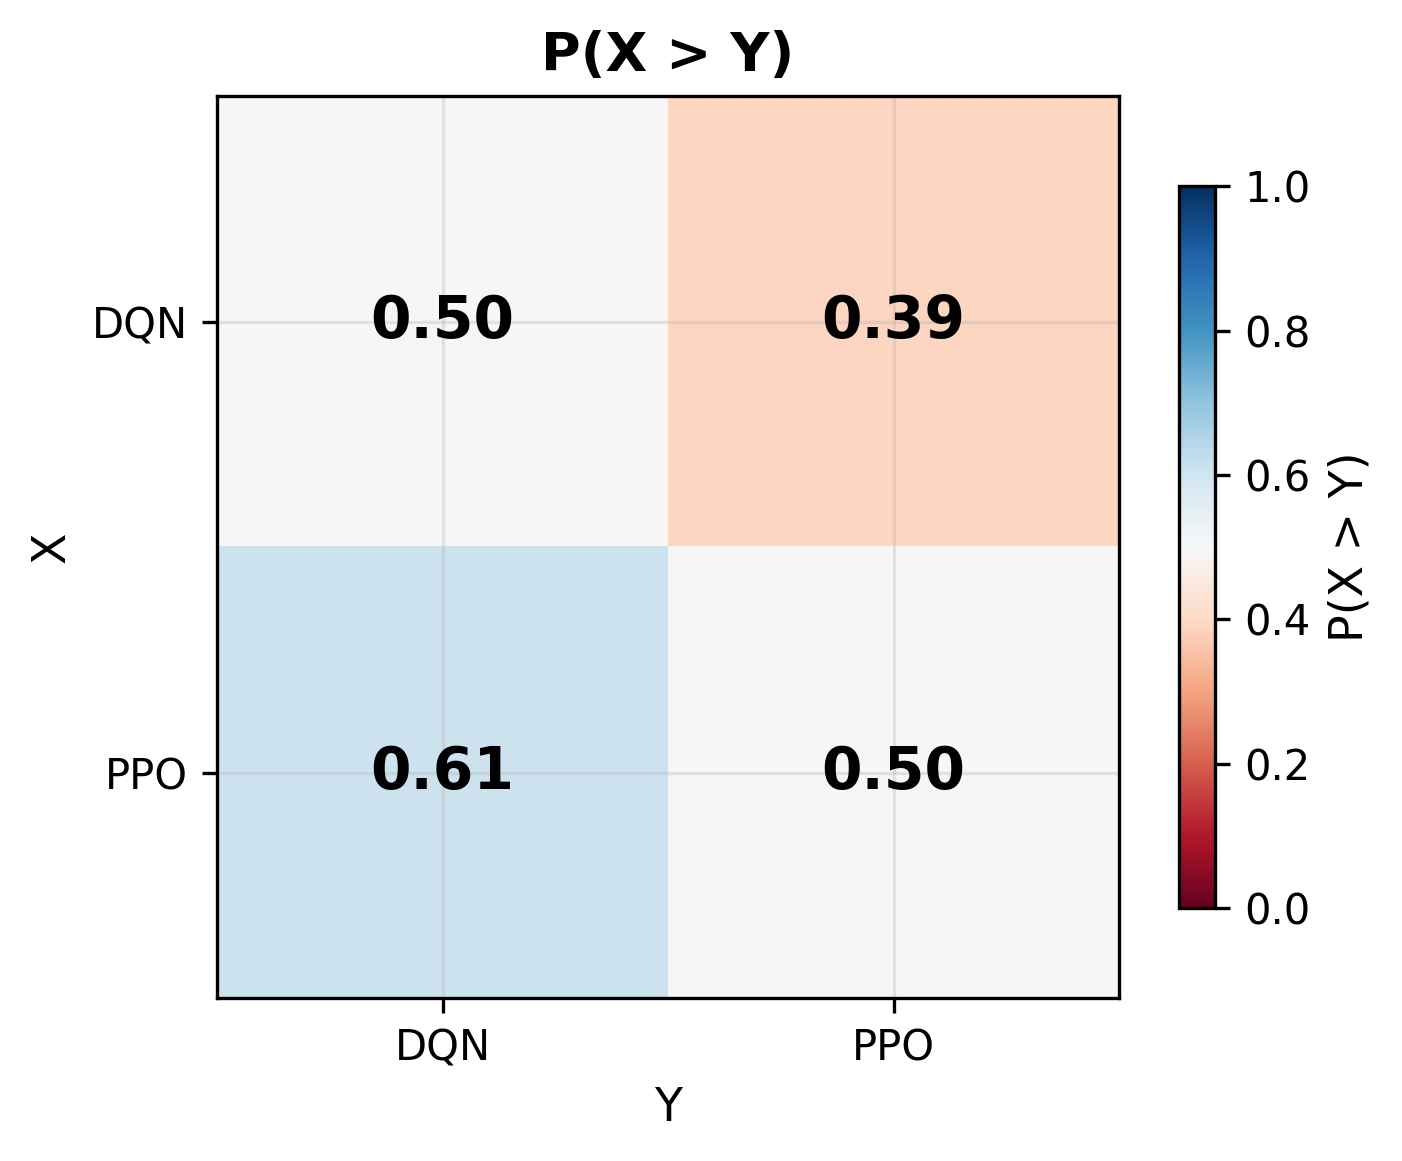
\includegraphics[width=0.8\linewidth]{5_exp2_atari/assets/poi_heatmap.png}
  \caption[Probability of improvement: Pong and Breakout]{Probability-of-improvement heatmap. PPO wins overall
           ($0.648$), but not overwhelmingly---DQN's Breakout edge
           prevents a decisive margin.}
  \label{fig:atari-poi}
\end{figure}

\subsection{Wall-Clock Timing Analysis}
\label{sec:atari-timing}

Training times are reported in Table~\ref{tab:atari-training-time}
(Section~\ref{sec:atari-training}). Here I focus on evaluation timing.
Figure~\ref{fig:atari-timing} shows the evaluation timing breakdown.
PPO evaluation took $1{,}256$\,s total ($823$\,s Pong, $434$\,s
Breakout); DQN evaluation took $2{,}133$\,s total ($1{,}704$\,s Pong,
$429$\,s Breakout). DQN's Pong evaluation is disproportionately slow
because lower scores mean longer episodes (the opponent scores points
more slowly when the agent puts up some resistance, but not enough
to win quickly).

Combining training and evaluation, the total wall-clock cost of
Experiment~2 was approximately $190{,}462$\,s (${\approx}53$\,h):
$99{,}329$\,s for PPO and $91{,}164$\,s for DQN. Training dominates
the budget---evaluation accounts for less than 2\% of the total.

\begin{figure}[htbp!]
  \centering
  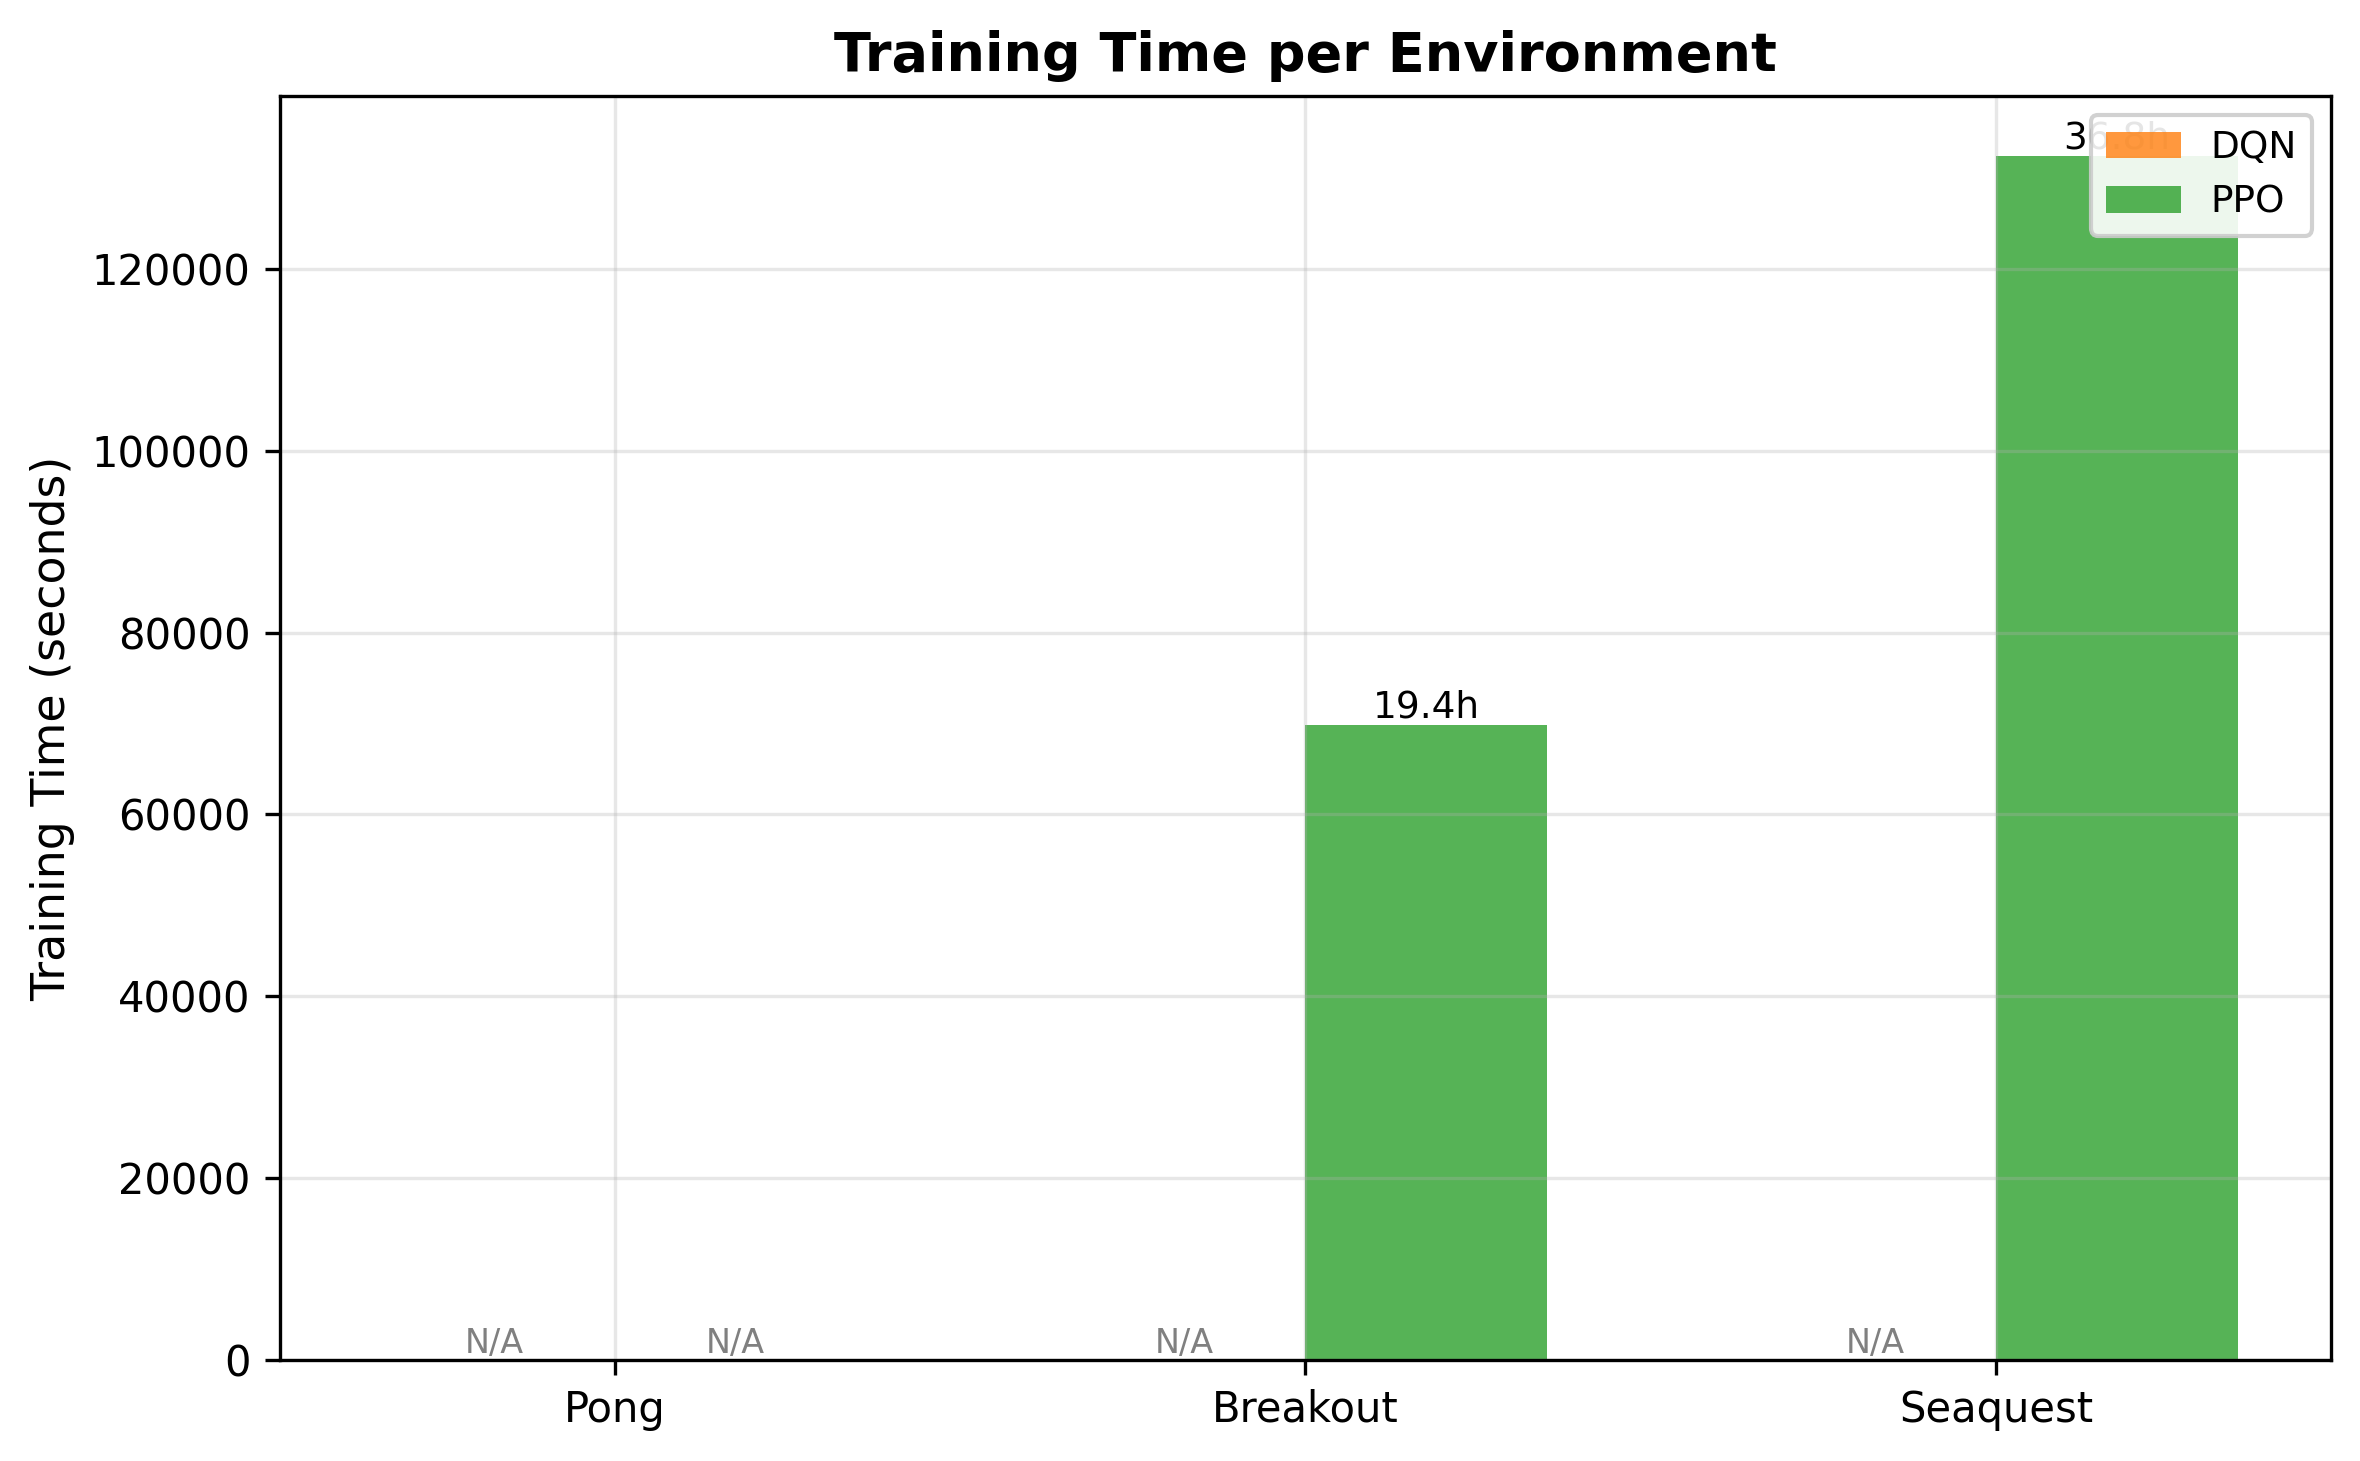
\includegraphics[width=\linewidth]{5_exp2_atari/assets/timing_analysis.png}
  \caption[Training time: Pong and Breakout]{Wall-clock evaluation time per algorithm and environment.
           DQN Pong evaluation is slowest due to longer episodes from
           intermediate-skill play.}
  \label{fig:atari-timing}
\end{figure}

%% ------------------------------------------------------------------
\section{Key Findings: Expectations vs Reality}
\label{sec:atari-key-findings}

Looking back at the hypotheses in Section~\ref{sec:atari-hypotheses},
the results again contained both confirmations and surprises.

\paragraph{PPO Pong dominance was expected---the margin was striking.}
I expected PPO to perform well on Pong, but IQM $0.983$ with an IQR
of just $1.08$ raw-return units across all 10 seeds is remarkable
consistency. PPO essentially solves Pong. By contrast, DQN achieves
IQM $0.217$ with a spread from $-18.90$ to $+10.72$. The gap between
PPO's worst seed ($17.90$) and DQN's best ($10.72$) is larger than
DQN's entire IQR. PPO's clipped surrogate objective handles Pong's
simple $\pm1$ reward structure with the same robustness it showed on
classic-control tasks.

\paragraph{DQN Breakout advantage---the surprise.}
I expected DQN to excel on Breakout, and it does edge PPO ($43.62$
vs $32.51$ mean return), but the margin is smaller than anticipated.
DQN's experience replay allows it to revisit rare brick-destruction
trajectories that PPO discards after each gradient step. However,
both algorithms achieve less than 11\% of the maximum score ($400$),
suggesting that 5M steps is insufficient for either algorithm to
develop the paddle-positioning strategies needed for deep brick
penetration.

\paragraph{Neither algorithm solves Breakout.}
{\color{red} Both algorithms are still learning on Breakout at 5M steps --- neither has converged. DQN reaches 43.62 and PPO reaches 32.51 under SB3 default hyperparameters. \citet{defuente2024comparative} report DQN reaching approximately 280 and PPO approximately 175 at the same budget with tuned configurations, confirming that DQN holds a task-specific advantage on Breakout at this scale --- its experience replay allows direct exploitation of the brick-breaking reward structure that suits Q-value estimation well. The gap between our scores and theirs reflects the cost of default settings, not a fundamental ceiling. \citet{mnih2015human} established the longer-run benchmark at 401.2 using 50 million frames, a replay buffer ten times larger than the SB3 default, and hyperparameters informally tuned on Breakout specifically (see Section~\ref{subsec:experimental-design}).}

\paragraph{POI is not decisive.}
$P(\text{PPO} > \text{DQN}) = 0.648$ is far less clear-cut than
Experiment~1's PPO dominance ($P > 0.89$ against all). With only
$M = 2$ environments, a single environment win heavily influences
the aggregate. PPO's Pong dominance and DQN's Breakout edge largely
cancel out in the probability calculation.

\paragraph{Cross-environment aggregates are misleading with $M = 2$.}
PPO's cross-environment IQM ($0.529$) is heavily influenced by its
near-perfect Pong scores pulling up the average, masking the fact
that DQN actually outperforms PPO on Breakout. With only two
environments, the IQM is essentially the average of one very high
score and one very low score---a number that describes neither
environment accurately.

%% ------------------------------------------------------------------
{\color{red} \section{Threats to Validity}}
\label{sec:atari-threats}

Several limitations constrain the generalisability of these results:
\begin{itemize}
  \item \textbf{Small environment suite ($M = 2$).} Even fewer
        environments than Experiment~1's $M = 3$. Cross-environment
        aggregates are extremely fragile---a single environment swap
        could reverse the overall ranking
        \citep{agarwal2021precipice, patterson2024edrl}.
  \item \textbf{Insufficient training budget.} The original DQN paper
        \citep{mnih2015human} used 50M frames (${\sim}12.5$M steps);
        our 5M-step budget may leave both algorithms undertrained,
        particularly on Breakout.
  \item \textbf{Default hyperparameters.} No per-algorithm tuning was
        performed, the same caveat as Experiment~1. DQN's replay buffer
        size, learning rate, and exploration schedule were all left at
        SB3 defaults.
  \item \textbf{GPU non-determinism.} Unlike Experiment~1, bitwise
        reproducibility is not possible. Results depend on statistical
        validity from 10~seeds rather than deterministic verification.
\end{itemize}

\section{Discussion}
\label{sec:atari-discussion}

\paragraph{Comparison with Experiment~1.}
In Experiment~1, PPO dominated across all three classic-control
environments (cross-environment IQM $0.981$, $P > 0.89$ against
every competitor). In Experiment~2, PPO still leads overall (IQM
$0.529$ vs $0.130$), but the picture is more nuanced. I attribute
this to the observation space: pixel-based observations with
longer horizons and sparser rewards (Breakout) create conditions
where DQN's replay buffer provides a genuine advantage. I now
believe DQN's failure on classic-control was a budget issue---200K
steps with SB3's default $\varepsilon$-greedy schedule was
insufficient. On Atari with 5M steps, DQN has enough data to show
its strengths, at least on Breakout.

\paragraph{Methodological notes.}
The standard Atari wrapper stack includes \texttt{ClipRewardEnv},
which clips all rewards to $\{-1, 0, +1\}$ during training. This
is beneficial for learning stability but means that naive evaluation
(reading rewards from the training environment) would report clipped
scores rather than true game returns. The fresh evaluation pipeline
uses SB3's \texttt{evaluate\_policy()}, which reads the true episode
returns from the \texttt{Monitor} wrapper, bypassing
\texttt{ClipRewardEnv}. This distinction was critical for obtaining
meaningful Breakout scores.

\paragraph{Future work.}
Several directions would strengthen these findings:
\begin{itemize}
  \item \textbf{Extend training budget}: run both algorithms for 10M
        or 50M steps to test whether Breakout performance improves
        substantially with more data.
  \item \textbf{Add more Atari environments}: SpaceInvaders, Seaquest,
        and BeamRider would increase $M$ and make cross-environment
        aggregates more meaningful.
  \item \textbf{Hyperparameter tuning}: test DQN with adjusted replay
        buffer size, learning rate, and exploration schedule to
        determine whether its Pong failure is a hyperparameter artefact.
  \item \textbf{Include additional algorithms}: A2C and QR-DQN on
        Atari for a fuller family comparison.
  \item \textbf{Continuous-action environments}: MuJoCo tasks with
        SAC and TD3 would provide a third experiment bridging the
        discrete-vs-continuous divide.
  \item \textbf{Fair budget comparison}: wall-clock normalised
        analysis (performance per compute hour) would account for
        the different computational costs of on-policy vs off-policy
        training.
\end{itemize}
